\documentclass[spanish,xcolor=table]{beamer}
\usepackage[spanish]{babel}
\selectlanguage{spanish}
\usepackage[utf8]{inputenc}
\mode<presentation> {

%----------------Beamer Themes--------------------

\usetheme{Boadilla}

%--------------------Beamer Font & Colors----------

\usecolortheme{seahorse}

%-------------------Beamer Options --------------------

\setbeamertemplate{navigation symbols}{} % To add the navigation symbols from the bottom of all slides comment this line
}

%-------------------Package----------------------------
\RequirePackage{natbib}
\usepackage{graphicx} 
\usepackage{booktabs} % use of \toprule, \midrule and \bottomrule in tables
\usepackage{tikz}
\usepackage{pgfplots}
\usepackage{multirow}
\usepackage{multicol}
\usepackage{amsmath}
\usepackage{hhline}
\usepackage[export]{adjustbox} %para posicionar imagenes(ej, left, right)

%---Librerias de Tikz -----------------------------
\usetikzlibrary{arrows,calc}
\usetikzlibrary{intersections}
\usetikzlibrary{pgfplots.fillbetween}
\usetikzlibrary{patterns}
\usetikzlibrary{plotmarks}
\usetikzlibrary{calc}
\usetikzlibrary{matrix}
\usetikzlibrary{positioning}
\usepackage{relsize}
\usepackage[nointegrals]{wasysym}
\usepackage{caption}
\usepackage{bigints}
\usepackage{xcolor}
%---------------------------------------------------------------------------------

%-----------Tikz Layers---------------------------------
\pgfdeclarelayer{ft}
\pgfdeclarelayer{bg}
\pgfsetlayers{bg,main,ft}
%---------------------------------------------------------


%--------Definiciones de Operadores --------------
\DeclareMathOperator*{\argmax}{arg\,max}
\def\checkmarkt{\tikz\fill[scale=0.4](0,.35) -- (.25,0) -- (1,.7) -- (.25,.15) -- cycle;} 
\newcommand{\bigqm}[1][1]{\text{\larger[#1]{\textbf{?}}}}
\let\Tiny=\tiny % fix issue font name beamer
\makeatletter

\newcommand\mathcircled[1]{%
  \mathpalette\@mathcircled{#1}%
}
\newcommand\@mathcircled[2]{%
  \tikz[baseline=(math.base)] \node[draw,circle,inner sep=1pt] (math) {$\m@th#1#2$};%
}

%north west lines pattern density ajusted
\pgfdeclarepatternformonly[\LineSpace,\LineSpaceColor]{MNWL}{\pgfqpoint{-1pt}{-1pt}}{\pgfqpoint{\LineSpace}{\LineSpace}}{\pgfqpoint{\LineSpace}{\LineSpace}}%
{
    \pgfsetcolor{\tikz@pattern@color}
    \pgfsetlinewidth{0.4pt}
    \pgfpathmoveto{\pgfqpoint{0pt}{\LineSpace}}
    \pgfpathlineto{\pgfqpoint{\LineSpace + 0.1pt}{-0.1pt}}
    \pgfsetstrokecolor{\LineSpaceColor}%        % <-- added
    \pgfusepath{stroke}
}
\makeatother

\newdimen\LineSpace
\tikzset{
    line space/.code={\LineSpace=#1},
    line space=6pt, %this ajust density of MNWL
    line color/.store in=\LineSpaceColor,      % <-- added
    line color=black,
} %line set color in custom parttern check line 665-667 for an example

%----------------------------------------------------------------------------------------
%	           Slide Inicial
%----------------------------------------------------------------------------------------
 

\title[ECO -TS101]{Econometr\'\i{}a de Series de Tiempo} 
\subtitle{T\'opico II.- Univariate Time Series Models}

%Profesores

\author{Marcelo Villena Ch., PhD} 

%-----------------------------------------------------------------

\institute[UAI] % Your institution as it will appear on the bottom of every slide, may be shorthand to save space
{
Universidad Adolfo Ib\'a\~nez 
 \\ % institution for the title page
\medskip
}
\date{} % Date, can be changed to a custom date

%-------------------Figure Settings-------------------
\pgfplotsset{ % Here we specify options for all figures in the document
  compat=1.8, % Which version of pgfplots do we want to use?
  legend style = {font=\small\sffamily}, % Legends in a sans-serif font
  label style = {font=\small\sffamily} % Labels in a sans-serif font
}

%-----Color definitions-------------
\colorlet{ColorG}{black!60!green}
\colorlet{ColorR}{black!60!red}
\colorlet{ColorB}{black!60!blue}
\colorlet{ColorY}{black!40!yellow}
%-----------------------------------

\begin{document}

\begin{frame}

\begin{figure}[t!]

\includegraphics[scale=0.1]{Logo.jpg}
\end{figure}
\titlepage % Print the title page as the first slide
\end{frame}

\begin{frame}
\frametitle{Contenidos} 
\tableofcontents % Lista de contenidos, carga la instruccion \section{} y \subsection{} 
\end{frame}


%----------------------------------------------------------------------------------------
%	PRESENTATION SLIDES
%----------------------------------------------------------------------------------------

%------------Slides------------------------------------
%---------------------Slide 3--------------------------

\begin{frame}
\frametitle{Ejemplo de repaso clase anterior\newline
Detrending global temperature}
Como vimos en la clase anterior, la evoluci\'on de la temperatura global manifestaba una tendencia lineal, por lo que podemos asumir que esta puede ser escrita como:
\begin{equation*} 
x_t =\mu_{t} + y_t
\end{equation*}
 Veremos dos maneras de de descomponer la serie, ``filtrando" la tendencia.
\end{frame}

%---------------------------------------------------------
%---------------------Slide 4 --------------------------
\begin{frame}
\frametitle{Ejemplo de repaso clase anterior\newline
Detrending global temperature}

\only<1|handout:1>{
\begin{exampleblock}{C\'odigo en R}
rm(list=ls())\\
mydata$<-$read.csv (``gtemp.csv")\\
gtemp$<-$mydata$\$$``gtem"\\
plot(gtemp, type=``o", ylab= ``Global Temperature Deviations'')\\
t$<-$1:142\\
summary(reg $<-$ lm(gtemp $\string ~$ t))\\
plot(gtemp, type=``o", ylab=``Global Temperature Deviations'')\\
abline(reg)\\
\end{exampleblock}
}

\end{frame}
%---------------------------------------------------------
%---------------------Slide 5--------------------------
\begin{frame}
\frametitle{Ejemplo de repaso clase anterior\newline
Detrending global temperature}

\begin{figure}[t!]
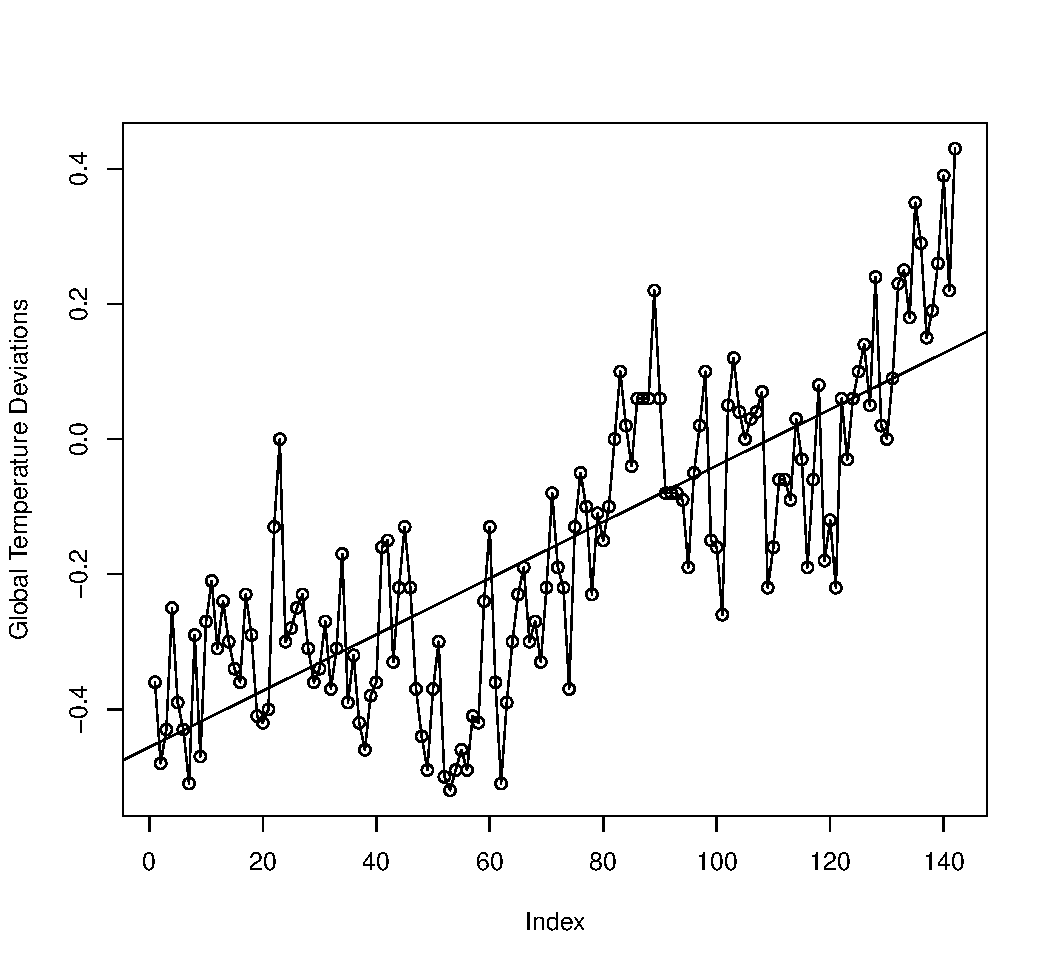
\includegraphics[scale=0.25]{gtemp_graph.pdf}
\end{figure}
 
\end{frame}

%---------------------------------------------------------
%---------------------Slide 6--------------------------
\begin{frame}
\frametitle{Ejemplo de repaso clase anterior\newline
Detrending global temperature}

\begin{figure}[t!]
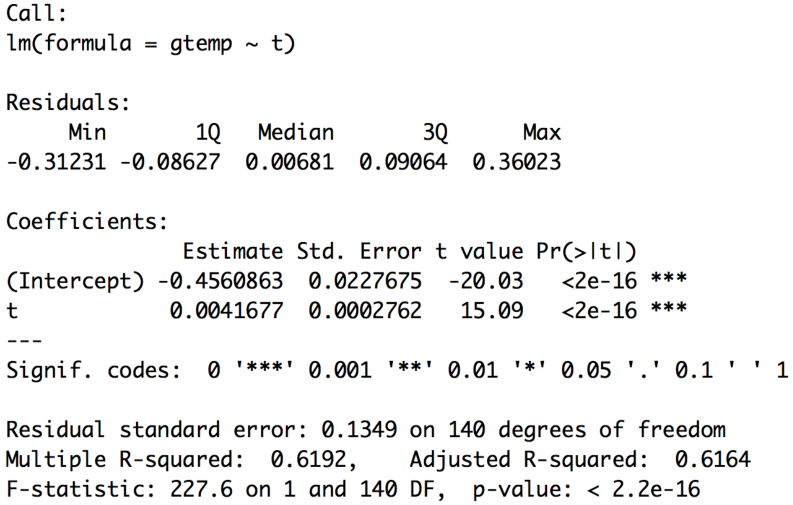
\includegraphics[scale=0.5]{reg_ej1.png}
\end{figure}
 
\end{frame}

%---------------------------------------------------------
%---------------------Slide 7 --------------------------
\begin{frame}
\frametitle{Ejemplo de repaso clase anterior\newline
Detrending global temperature}

\only<1|handout:1>{
\begin{exampleblock}{C\'odigo en R}
reg1= lm(gtemp$\string ~$ time(gtemp), na.action=NULL) \\
par(mfrow=c(2,1))\\
plot(resid(reg1), type=``o", main=``detrended")\\
plot(diff(gtemp), type=``o", main=``first difference")\\
\end{exampleblock}
}

\end{frame}
%---------------------------------------------------------
%---------------------Slide 8--------------------------
\begin{frame}
\frametitle{Ejemplo de repaso clase anterior\newline
Detrending global temperature}

\begin{figure}[t!]
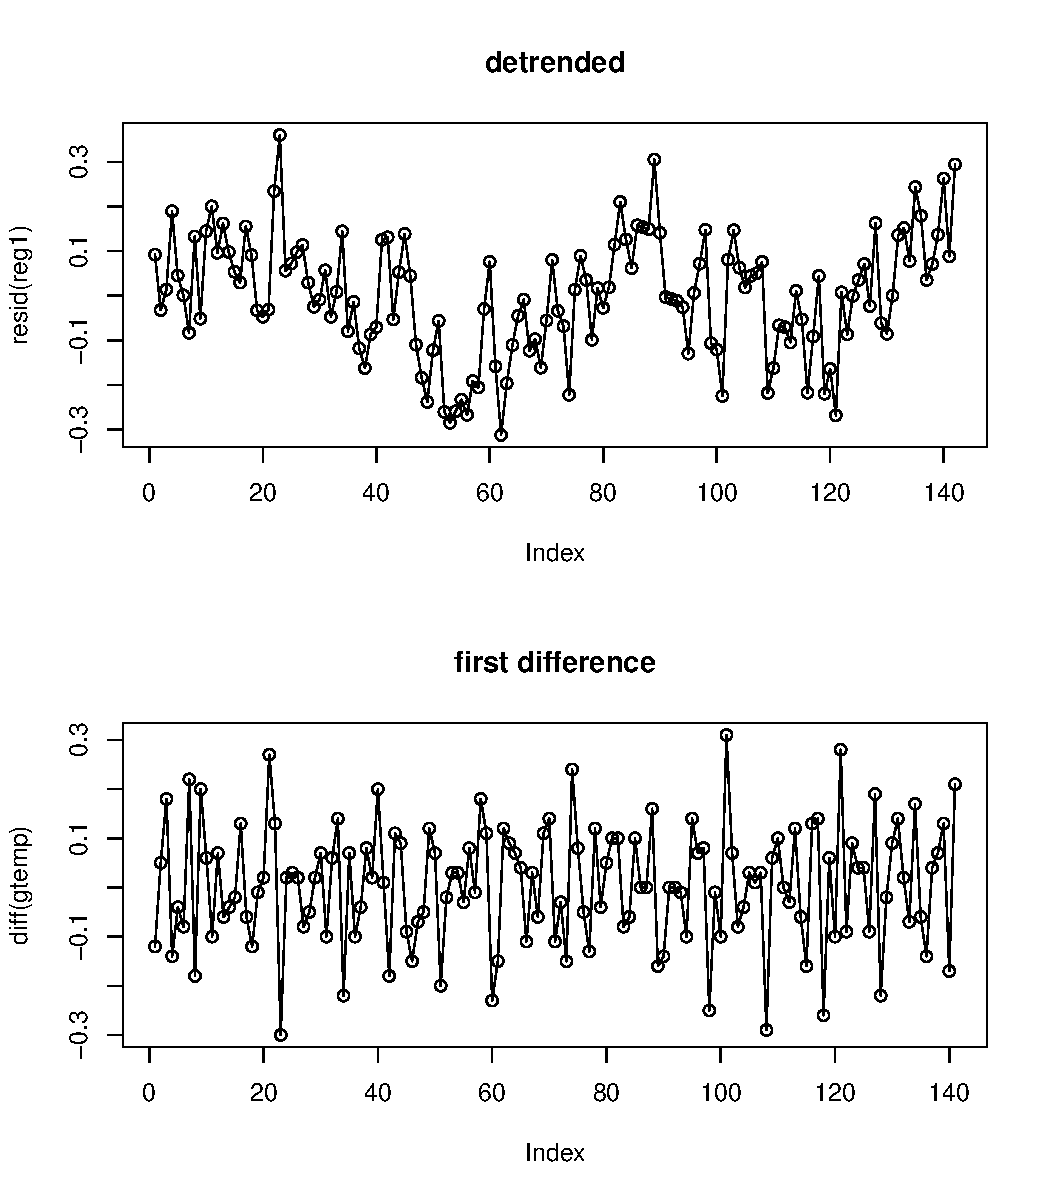
\includegraphics[scale=0.25]{detrended.pdf}
\end{figure}
 
\end{frame}

%---------------------------------------------------------
%---------------------Slide 9 --------------------------
\begin{frame}
\frametitle{Ejemplo de repaso clase anterior\newline
Detrending global temperature}

\only<1|handout:1>{
\begin{exampleblock}{C\'odigo en R}
par(mfrow=c(3,1)) \\
acf(gtemp, 48, main=``gtemp")\\
acf(resid(reg), 48, main=``detrended")\\
acf(diff(gtemp), 48, main=``first difference")\\
\end{exampleblock}
}

\end{frame}
%---------------------------------------------------------
%---------------------Slide 10--------------------------
\begin{frame}
\frametitle{Ejemplo de repaso clase anterior\newline
Detrending global temperature}

\begin{figure}[t!]
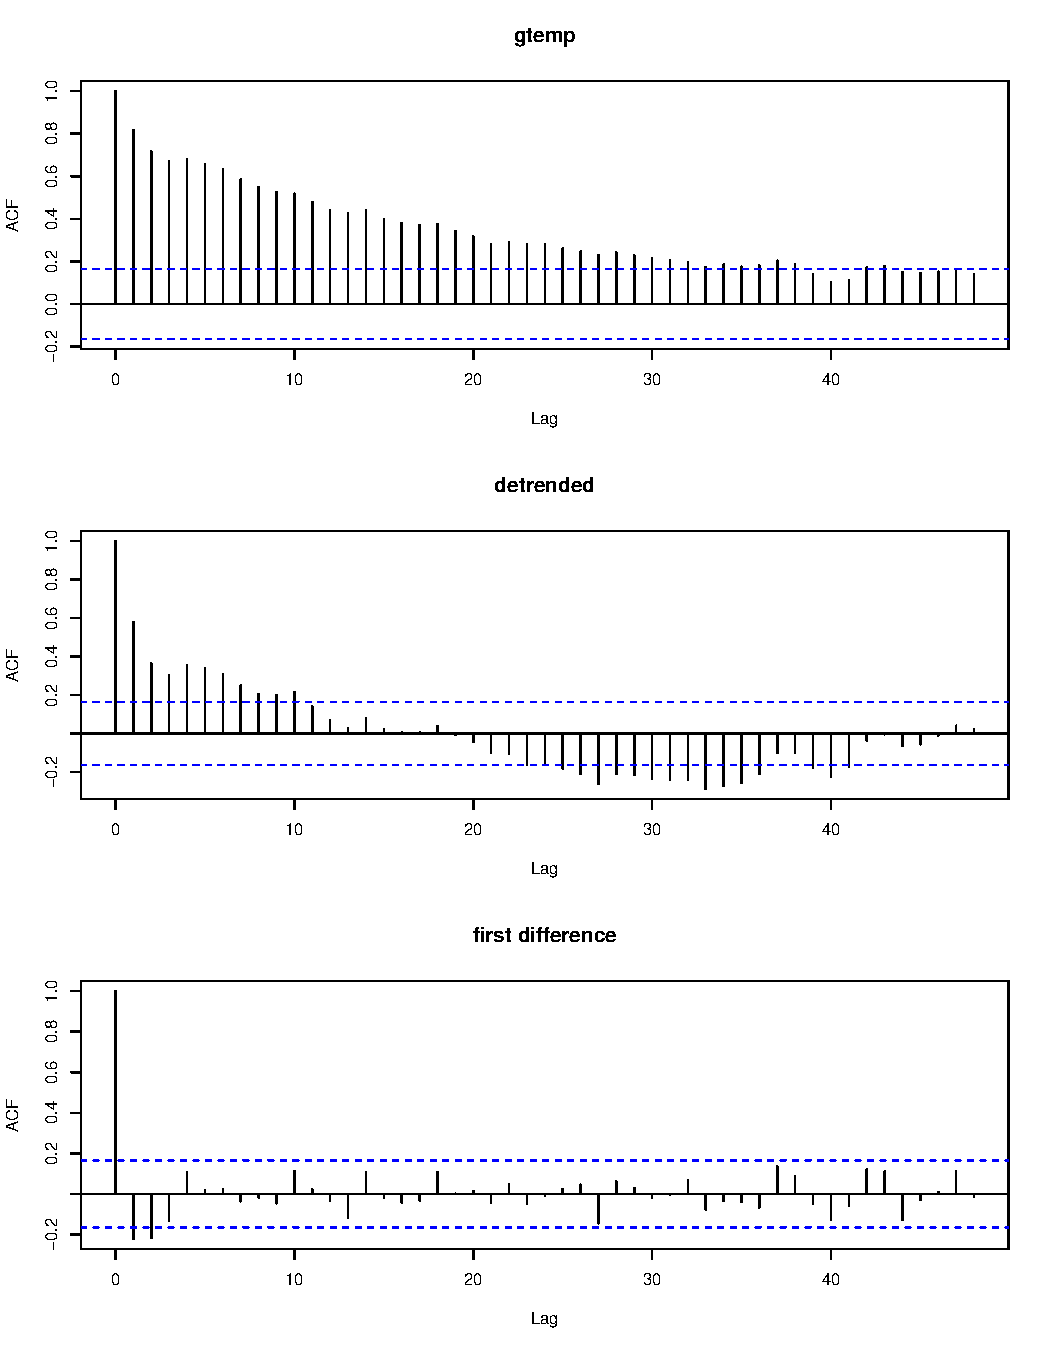
\includegraphics[scale=0.25]{acf_example1.pdf}
\end{figure}
 
\end{frame}

%---------------------------------------------------------
%---------------------Slide 11--------------------------
\begin{frame}
\frametitle{Sobre la descomposici\'on de una serie}

En los gr\'aficos podemos apreciar que la primera diferencia de la serie produce resultados diferentes a la eliminaci\'on de la tendencia mediante la regresi\'on de la tendencia.\\
En el caso de los gr\'aficos ACF, el proceso diferenciado muestra una autocorrelaci\'on mi\'{\i}nima, lo que puede implicar que la serie de temperatura global es similar una caminata aleatoria con deriva.\\
Es interesante notar que si la serie es una caminata aleatoria con deriva, la media de la serie diferenciada, que es una estimaci\'on de la deriva, es aproximadamente $,0066$, pero con un gran error est\'andar:\\
\only<1|handout:1>{
\begin{exampleblock}{C\'odigo en R}
mean (diff (gtemp))\\
sd (diff (gtemp)) / sqrt (longitud (diff (gtemp)))
\end{exampleblock}
}
\end{frame}
%---------------------------------------------------------
%---------------------Slide 12--------------------------

\begin{frame}
\frametitle{Sobre la descomposici\'on de una serie}

Una ventaja de diferenciar sobre la estimaci\'on de una tendencia,  para eliminar las tendencias, es que no se estiman par\'ametros en la operaci\'on de diferenciaci\'on. Una desventaja, sin embargo, es que la diferenciaci\'on no arroja una estimaci\'on del proceso estacionario $y_t$.\\
\vspace{5mm}	 
De esta forma, si una estimaci\'on de $y_t$ es esencial, entonces la estimaci\'on de una tendencia puede ser la forma m\'as apropiada para eliminar las tendencias de la serie. Si el objetivo es forzar los datos a la estacionaridad, entonces la diferenciaci\'on puede ser m\'as apropiada. La diferenciaci\'on tambi\'en es una herramienta viable si la tendencia es fija.\\
 \vspace{3mm}	
 En EE.UU. el procedimiento oficial de descomposici\'on y ajuste estacional se llama:\\
 \vspace{3mm}	
 \textbf{X-13-ARIMA (http://www.census.gov/srd/www/x13as/)}

\end{frame}

%---------------------------------------------------------
%---------------------Slide 13--------------------------

\begin{section}{Procesos no estacionarios, integrados y el test de ra\'{\i}z unitaria}
\begin{frame}
\frametitle{Procesos no estacionarios, integrados y el test de ra\'{\i}z unitaria}

Recordemos que si una serie de tiempo es estacionaria, su media, su varianza y su autocovarianza (en diferentes rezagos) permanecen iguales sin importar el momento del tiempo en el cual se midan; es decir, son \textbf{invariantes respecto al tiempo}.
\par
Por otro lado, hemos visto que la estacionaridad es una caracter\'{\i}stica deseable, por ejemplo, en t\'erminos de la normalidad de las variables. Sin embargo, en la pr\'actica nos encontramos con:
\par
\only<1->{
\begin{itemize}
\item[(i)] Procesos No-estacionarios: Cuando un proceso estoc\'astico de series de tiempo es dependiente del tiempo.
\item[(ii)] Procesos Integrados: un proceso no-estacionario, el cual puede ser transformado a proceso estacionario diferenciando.
\end{itemize}
}
 
\end{frame}

%---------------------------------------------------------
%---------------------Slide 14--------------------------
\begin{frame}
\frametitle{Procesos Integrados}

Con respecto a los Procesos Integrados, partimos definiendo:
\only<1->{
\begin{itemize}
\item La secuencia $\{x_t\}$ es integrada de orden $d$, $I(d)$, si esta requiere ser diferenciada $d$ veces para llegar a ser estacionaria.
\item Todos los \textbf{Procesos Integrados son no-estacionarios}, pero no todos los procesos no-estacionarios son integrados.
\item Si la secuencia $\{x_t\}$  tiene una ra\'{\i}z unitaria, entonces, es un proceso integrado, y de aqu\'{\i} no-estacionario.
\end{itemize}
}
 
\end{frame}

%---------------------------------------------------------
%---------------------Slide 15--------------------------
\begin{frame}
\frametitle{Consecuencias de los Procesos Integrados (Ra\'{\i}z Unitaria)}

\only<1->{
\begin{itemize}
\item Es importante se\~nalar que los test estad\'{\i}sticos est\'andares no son apropiados cuando los MCO (OLS) son aplicados a procesos integrados, ver por ejemplo \cite{granger1974spurious}.
\item Si la secuencia $\{x_t\}$ es un proceso de ra\'{\i}z unitaria, entonces, cualquier shock tiene un efecto permanente (que no decae). De aqu\'{\i}, la serie de tiempo es modelada apropiadamente suponiendo una tendencia estoc\'astica. La serie de tiempo entonces puede ser definida como estacionaria diferenciable, y se le deber\'a sacar la tendencia diferenciando. 
\item En este contexto, \textbf{los t\'erminos no-estacionariedad, caminata aleatoria, ra\'{\i}z unitaria y tendencia estoc\'astica se consideran sin\'onimos}. 
\end{itemize}
}
 
\end{frame}

%---------------------------------------------------------
%---------------------Slide 16--------------------------
\begin{frame}
\frametitle{Test de Ra\'{\i}z Unitaria}

Considere el siguiente proceso autoregresivo:

\begin{equation} \label{AR1}
x_t =\alpha_1 x_{t-1} + \epsilon_t
\end{equation}

Si $\alpha_1=1$, la secuencia $x_t$ es una ra\'{\i}z unitaria.

El test est\'andar para probar esta hip\'otesis, consiste en restar $x_{t-1}$ a la ecuaci\'on anterior de forma que:

\begin{equation}
\triangle x_t =\gamma x_{t-1} + \epsilon_t
\end{equation}

donde $\gamma=\alpha_1-1$, y $\triangle x_t = x_t - x_{t-1}$. En este contexto, probar la hip\'otesis que la ecuaci\'on (1) tiene una ra\'{\i}z unitaria, $\alpha_1 = 1$, es equivalente a probar la hip\'otesis de $\gamma=0$ en ecuaci\'on (2). 
Este es b\'asicamente el enfoque de Dickey-Fuller (DF) para ra\'{\i}ces unitarias, ver por ejemplo \cite{dickey1981likelihood}. Adicionalmente existe el test aumentado de Dickey-Fuller (ADF), y muchos otros tests que se basan el l\'ogicas similares, y que utilizaremos durante el curso.

\end{frame}

%---------------------------------------------------------
%---------------------Slide 17 --------------------------
\begin{frame}
\frametitle{Ejemplo de Test de Ra\'{\i}z Unitaria - Dickey-Fuller}

\only<1|handout:1>{
\begin{exampleblock}{C\'odigo en R}
install.packages(``tseries")\\
library(tseries)\\
adf.test(gtemp)\\
adf.test(resid(reg1))\\
adf.test(diff(gtemp))\\
\end{exampleblock}
}

\end{frame}
%---------------------------------------------------------
%---------------------Slide 18 --------------------------
\begin{frame}
\frametitle{Ejemplo de Test de Ra\'{\i}z Unitaria - Dickey-Fuller}

Augmented Dickey-Fuller Test\\
data:  gtemp\\
Dickey-Fuller = -2.0624, Lag order = 5, p-value =
0.5505\\
alternative hypothesis: stationary\\
\vspace{5mm}	    
Augmented Dickey-Fuller Test\\
data:  resid(reg1)\\
Dickey-Fuller = -2.0624, Lag order = 5, p-value =
0.5505\\
alternative hypothesis: stationary\\
\vspace{5mm}	    
Augmented Dickey-Fuller Test\\
data:  diff(gtemp)\\
Dickey-Fuller = -6.8179, Lag order = 5, p-value = 0.01\\
alternative hypothesis: stationary\\
\end{frame}

\end{section}
%---------------------------------------------------------
%---------------------Slide 19--------------------------
\begin{section}{Modelos ARIMA: modelando el corto plazo}
\begin{frame}
\frametitle{Modelos ARIMA: modelando el corto plazo}

En el a\~no 1970, la metodolog\'{\i}a propuesta por George Box y Gwilym Jenkins, \cite{BoxJenkins} , dos ingenieros con formaci\'on estad\'{\i}stica sistematizan modelos estad\'{\i}sticos para el an\'alisis de series temporales univariantes, teniendo en cuenta para esto la dependencia existente entre los datos. \\
As\'{\i}, cada observaci\'on es modelada en funci\'on de los valores anteriores, la variable tiempo, por tanto, juega un papel fundamental. 
 
\end{frame}

%---------------------------------------------------------
%---------------------Slide 20--------------------------
\begin{frame}
\frametitle{Modelos ARIMA: modelando el corto plazo}

Los modelos de predicci\'on de Box-Jenkins pertenecen a la familia de modelos alg\'ebraicos lineales, que consideran que una serie temporal real constituye una probable realizaci\'on de un determinado proceso estoc\'astico.\\
\vspace{4mm}	
Estos modelos se conocen con el nombre gen\'erico de ARIMA (Auto-regresive Integrated Moving Average), el cual deriva de sus tres componentes Autoregresivo (AR), Integrado (I) de Medias M\'oviles (MA). Modelar una serie temporal supone identificar un modelo ARIMA adecuado que se ajuste a la serie objeto de estudio, debe contener los m\'{\i}nimos elementos necesarios para describir el fen\'omeno y ser \'util para realizar previsiones.
 
\end{frame}

%---------------------------------------------------------
%---------------------Slide 21--------------------------
\begin{frame}
\frametitle{Sobre el operador de retroceso - backshift operator}

\only<1|handout:1>{
\begin{block}{Definici\'on: operador de retroceso (backshift operator) }
Definimos el operador de retroceso (backshift operator) como:

\begin{equation}
B x_t = x_{t-1} 
\end{equation}
\begin{equation}
B^2 x_t =  B(B x_t) = B x_{t-1} = x_{t-2}
\end{equation}
As\'{\i}:
\begin{equation}
B^k x_t = x_{t-k} 
\end{equation}
\end{block}
}

De esta forma tenemos que la primera diferencia se puede definir en t\'erminos de lags, en otras palabras del operador de retroceso:
\begin{equation}
\triangle x_t = x_t - x_{t-1}= (1 - B) x_t 
\end{equation}
En general:
\begin{equation}
\triangle^d x_t = (1 - B)^d x_t 
\end{equation}

\end{frame}
%---------------------------------------------------------
%---------------------Slide 22--------------------------
\begin{frame}
\frametitle{Modelos ARIMA: modelando el corto plazo}

\only<1|handout:1>{
\begin{block}{Definici\'on: $AR (p)$}
Un modelo autorregresivo de orden p, frecuentemente abreviado como $AR(p)$, tiene la forma:
\begin{equation}
x_t = \phi_1 x_{t-1} +  \phi_2 x_{t-2} + \dots{} +  \phi_p x_{t-p} + \epsilon_t
\label{ar}
\end{equation}
donde $x_t$ es una serie estacionaria, y  $\phi_1$,  $\phi_2$,  \dots{} , $\phi_p$ son constantes. 
Si la media de $x_t$ es $\mu$, entonces podemos reemplazar $x_t-\mu$ en $\eqref{ar}$
\begin{equation}
x_t-\mu = \phi_1 (x_{t-1}-\mu) +  \phi_2 (x_{t-2}-\mu) + \dots{} +  \phi_p (x_{t-p}-\mu) + \epsilon_t
\end{equation}
\begin{equation}
x_t = \alpha + \phi_1 x_{t-1} +  \phi_2 x_{t-2} + \dots{} +  \phi_p x_{t-p} + \epsilon_t
\end{equation}
donde $\alpha = \mu(1-\phi_1-\phi_2\dots{}\phi_p)$\\
Usando los operadores de retroceso $AR(p)$ queda como:
\begin{equation}
(1- \phi_1 B + \phi_2 B^2 - \dots{}  - \phi_p B^p )
\end{equation}
o incluso m\'as concisamente
\begin{equation}
\phi (B) x_t = \epsilon_t
\end{equation}
\end{block}
}
 
\end{frame}

%---------------------------------------------------------
%---------------------Slide 23--------------------------
\begin{frame}
\frametitle{Ejemplo Proceso Autoregresivo de Orden 1: AR(1)}

En un procesos AR(1) la variable $x_t$ queda \'unicamente por su valor pasado $x_{t-1}$:
\begin{equation}
x_t = \phi x_{t-1} + \epsilon_t
\end{equation}

donde como sabemos $\epsilon_t$ es un proceso de ruido blanco con media cero y varianza constante $\sigma^2$, y $\phi$ es un par\'ametro. Para verificar que el modelo AR(1) es estacionario debemos probar que es:\\
\vspace{4mm}	
\textbf{(1) Estacionario en media}
\begin{equation}
E(x_t) = E(\phi x_{t-1} + \epsilon_t)=\phi E(x_{t-1} )
\end{equation}
Para que el proceso sea estacionario, la media debe ser constante y finita en el tiempo, lo que implica:
\begin{equation}
E(x_t) = \phi E(x_{t} )
E(x_t) = \frac{0}{1-\phi}=0
\end{equation}
\\
Por lo tanto, para que el proceso sea estacionario el par\'ametro $\phi \ne 0$.

\end{frame}

%---------------------------------------------------------
%---------------------Slide 24--------------------------
\begin{frame}
\frametitle{Ejemplo Proceso Autoregresivo de Orden 1: AR(1)}

\textbf{(2) Estacionario en covarianza}

Para verificar que el modelo AR(1) sea estacionario, la varianza debe ser constante y finita en el tiempo:

\begin{equation}
\gamma = E(x_t-E(x_t))^2 = E(\phi x_{t-1} + \epsilon_t - 0)^2 = \phi^2 var(x_{t-1}) + \sigma^2
\end{equation}

Asumiendo que el proceso es estacionario:
\begin{equation}
E(x_t)^2 = var(x_{t-1}) = var(x_{t}) = \gamma
\end{equation}
De aqu\'{\i} tenemos que:

\begin{equation}
\gamma  = \phi^2 \gamma + \sigma^2
\end{equation}

Por lo que:
\begin{equation}
\gamma  = \frac{\sigma^2}{1-\phi^2}
\end{equation}\\
Para que un proceso sea estacionario, varianza constante y finita, es necesario que $|\phi|< 1$.
\end{frame}

%---------------------------------------------------------
%---------------------Slide 25--------------------------
\begin{frame}
\frametitle{Ejemplo Proceso Autoregresivo de Orden 1: AR(1)}

Si se cumple que $|\phi|< 1$, entonces podemos representar el modelo AR(1) como un proceso lineal dado por:

\begin{equation}
x_t = \sum_{j=0}^{\infty} \phi^j \epsilon_{t-j}
\label{causal}
\end{equation}

La ecuaci\'on $\eqref{causal}$ se llama \textbf{soluci\'on estacionaria causal del modelo}. El t\'ermino causal se refiere al hecho de que $x_t$ no depende del futuro. De hecho, por simple sustituci\'on,\\
\begin{equation}
\underbrace{\sum_{j=0}^{\infty} \phi^j\epsilon_{t-j}}_{x_t} = \underbrace{\phi\left(\sum_{k=0}^{\infty} \phi^k\epsilon_{t-1-k}\right)}_{x_{t-1}}+\epsilon_t
\end{equation}

\end{frame}

%---------------------------------------------------------
%---------------------Slide 26 --------------------------
\begin{frame}
\frametitle{Simulaci\'on modelo AR(1) }

\only<1|handout:1>{
\begin{exampleblock}{C\'odigo en R}
par(mar=c(1,1,1,1))\\
par(mfrow=c(2,1))\\
plot(arima.sim(list(order=c(1,0,0), ar=.9), n=100), ylab=``x",\\
       main=(expression(AR(1)~~~phi==+.9)))\\
plot(arima.sim(list(order=c(1,0,0), ar=-.9), n=100), ylab=``x",\\
       main=(expression(AR(1)~~~phi==-.9)))\\
\end{exampleblock}
}

\end{frame}
%---------------------------------------------------------
%---------------------Slide 27 --------------------------
\begin{frame}
\frametitle{Simulaci\'on modelo AR(1) }

\begin{figure}[t!]
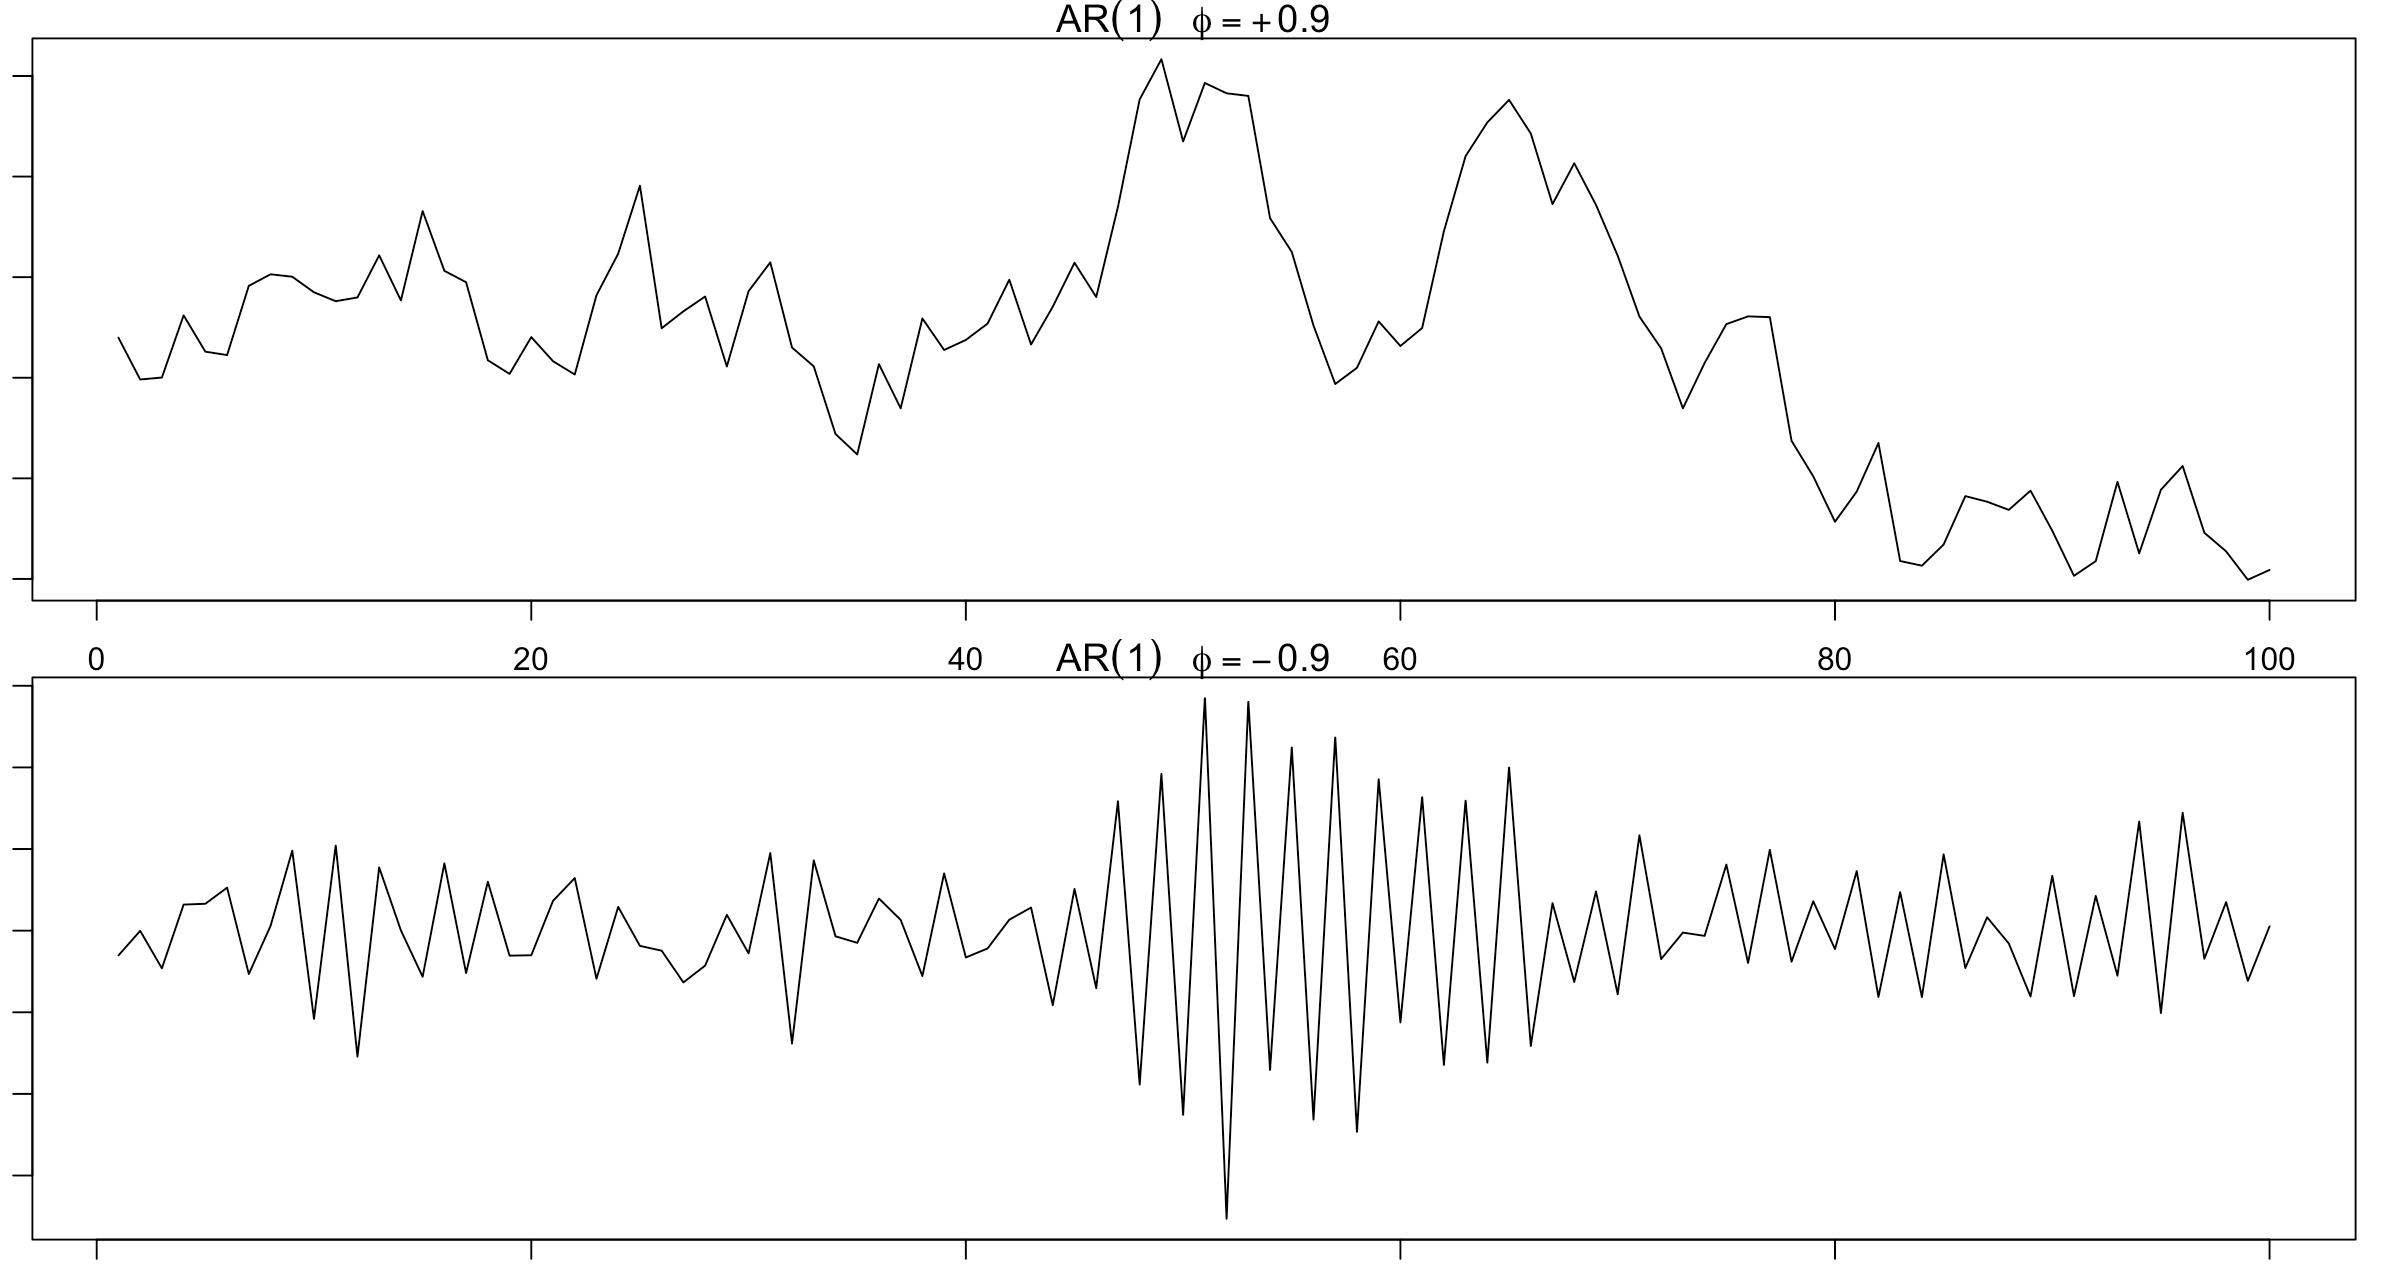
\includegraphics[scale=0.25]{ar.png}
\end{figure}
 
\end{frame}

%---------------------------------------------------------
%---------------------Slide 28--------------------------
\begin{frame}
\frametitle{Identificaci\'on modelo AR(1) }

Para el caso de un proceso del tipo AR, el correlograma, representaci\'on gr\'afica de la funci\'on de autocorrelaci\'on, tendr\'a un
comportamiento amortiguado hacia cero con todos los valores positivos, en caso de que $\theta > 0$, o bien alternando el signo, comenzando con negativo, si  $\theta < 0$.

\begin{figure}[t!]
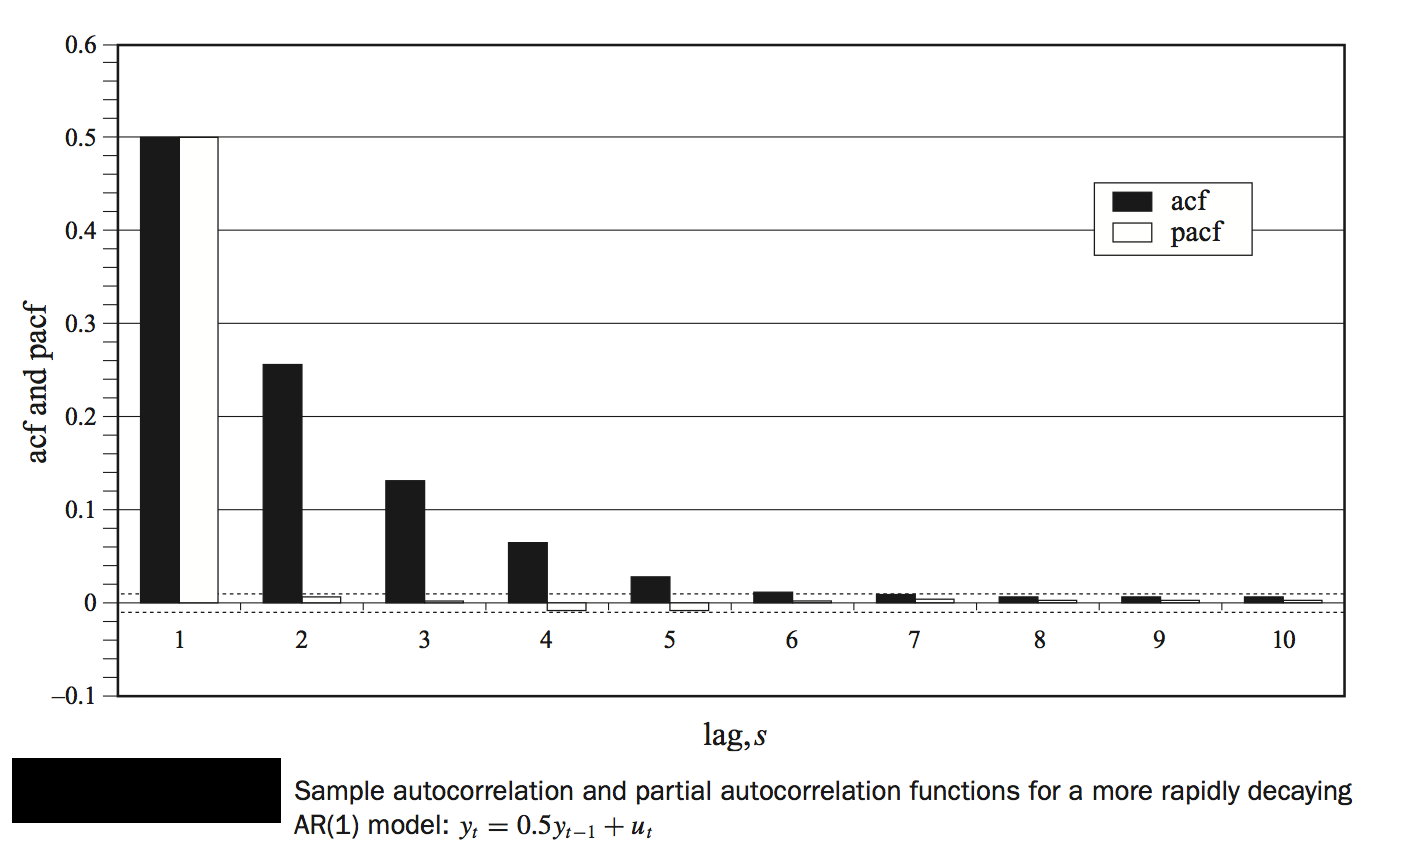
\includegraphics[scale=0.34]{ar1corr.pdf}
\end{figure}


\end{frame}
%---------------------------------------------------------
%---------------------Slide 29--------------------------
\begin{frame}
\frametitle{Identificaci\'on modelo AR(1) }
 
\begin{figure}[t!]
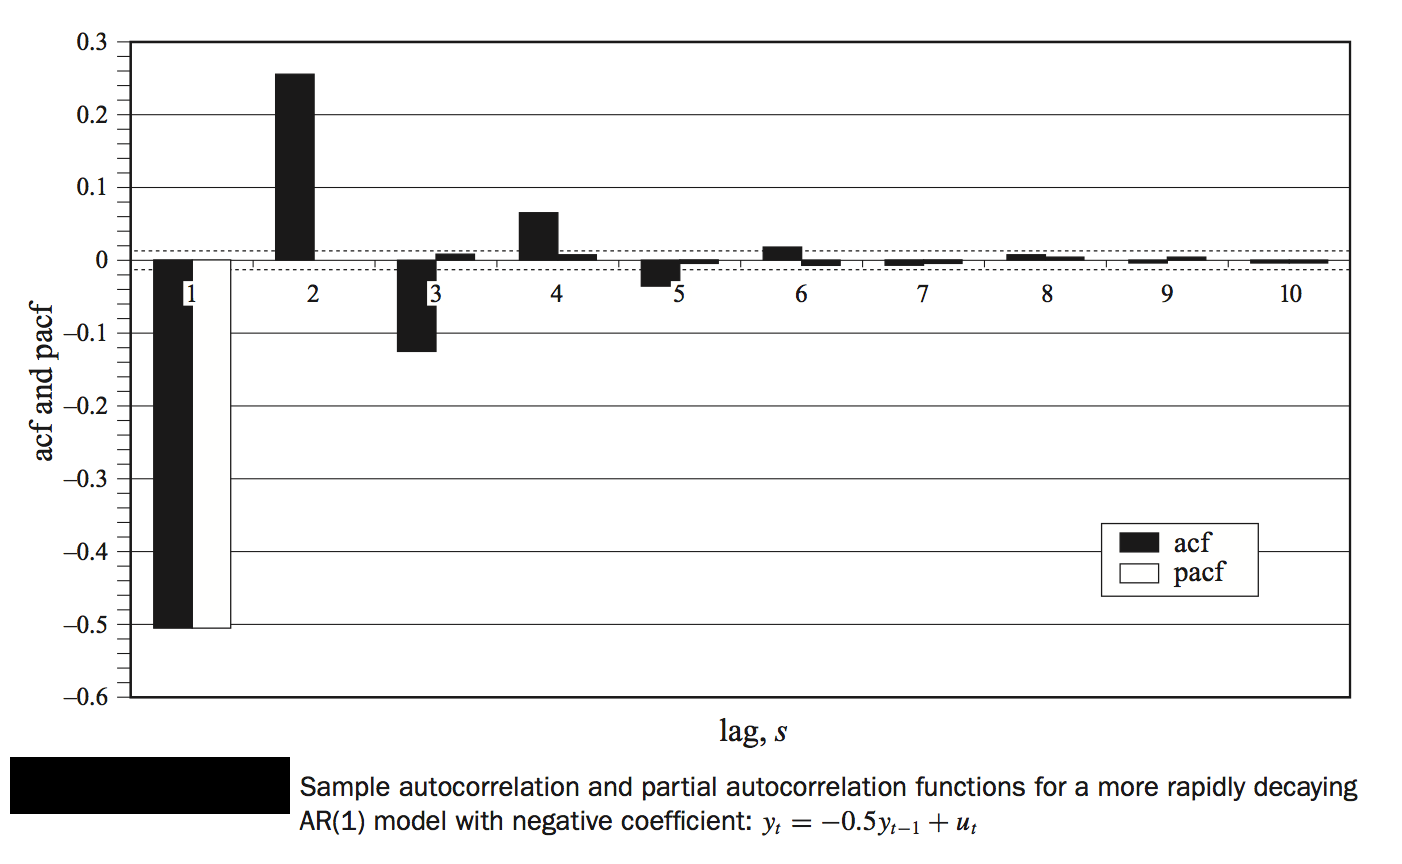
\includegraphics[scale=0.4]{ar1corrb.pdf}
\end{figure}

\end{frame}
%---------------------------------------------------------
%---------------------Slide 30--------------------------
\begin{frame}
\frametitle{Modelos ARIMA: modelando el corto plazo}

\textbf{Media M\'ovil - MA (q)}

Como una alternativa a la representaci\'on autorregresiva en la que se supone que el $x_t$ en el lado izquierdo de la ecuaci\'on se combina linealmente, el modelo de promedio m\'ovil de orden q, abreviado como $MA (q)$, asume que el ruido blanco $\epsilon_t$ usualmente a la mano derecha de la ecuaci\'on, se combinan linealmente para modelar los datos observados.

 
\end{frame}

%---------------------------------------------------------
%---------------------Slide 31--------------------------
\begin{frame}
\frametitle{Modelos ARIMA: modelando el corto plazo}

\only<1|handout:1>{
\begin{block}{Definici\'on: Media M\'ovil - $MA (q)$}
	
\begin{equation}
x_t = \epsilon_t + \theta_1 \epsilon_{t-1} +  \theta_2 \epsilon_{t-2} + \dots{} +  \theta_q \epsilon_{t-q} 
\end{equation}

donde hay $q$ rezagos de la media m\'ovil $\epsilon_t$ y $\theta_1$  + $ \theta_2$ + $\dots{}$ + $ \theta_q$ son par\'ametros. \\
\vspace{4mm}	
Aunque no es necesario, suponemos que $\epsilon_t$ es una serie de ruido blanco.

\end{block}
}
 
\end{frame}

%---------------------------------------------------------
%---------------------Slide 32--------------------------
\begin{frame}
\frametitle{Modelos ARIMA: modelando el corto plazo}

\only<1|handout:1>{
\begin{block}{Definici\'on: Media M\'ovil - $MA (q)$}

Tambi\'en podemos escribir el proceso $MA (q)$ en la forma equivalente:

\begin{equation}
x_t = \theta_t (B) \epsilon_{t} 
\end{equation}

donde  $\theta_t$ es el operador de promedio m\'ovil definido como:

\begin{equation}
\theta (B) = 1 + \theta_1B + \theta_2B^2 + \dots{} + \theta_q B^q
\end{equation}
\\
\vspace{4mm}	
A diferencia del proceso autorregresivo, el proceso de promedio m\'ovil es estacionario para cualquier valor de los par\'ametros $\theta_1$ + $\theta_2$ +$ \dots{}$ + $\theta_q$.


\end{block}
}
 
\end{frame}


%---------------------------------------------------------
%---------------------Slide 33--------------------------
\begin{frame}
\frametitle{Modelos ARIMA: modelando el corto plazo}

\textbf{Interpretaci\'on del model de media m\'ovil - MA (q)}

 As\'{\i} como un modelo autorregresivo es intuitivamente sencillo de comprender, la formulaci\'on de un modelo de medias m\'oviles resulta frecuentemente no intuitivo. ?`Qu\'e significa que una variable aleatoria se explique en funci\'on de los errores cometidos en per\'{\i}odos anteriores?, ?`De d\'onde vienen esos errores?, ?`Cu\'al es la justificaci\'on de un modelo de este tipo?.
En realidad, un modelo de medias m\'oviles puede obtenerse a partir de un modelo autorregresivo a partir de la realizaci\'on de sucesivas sustituciones.

\end{frame}

%---------------------------------------------------------
%---------------------Slide 34--------------------------
\begin{frame}
\frametitle{Modelos ARIMA: modelando el corto plazo}

\textbf{Interpretaci\'on del model de media m\'ovil - MA (q)}

Supongamos un modelo $AR(1)$, sin t\'ermino independiente:

\begin{equation}
x_t =  \phi x_{t-1} + \epsilon_t
\end{equation}

si consideramos $t-1$ en lugar de $t$ el modelo ser\'{\i}a en este caso:

\begin{equation}
x_{t-1} =  \phi x_{t-2} + \epsilon_{t-1}
\end{equation}

sustituyendo:

\begin{equation}
x_t =  \phi^2 x_{t-2} + \phi \epsilon_{t-1} + \epsilon_t
\end{equation}

\end{frame}

%---------------------------------------------------------
%---------------------Slide 35--------------------------
\begin{frame}
\frametitle{Modelos ARIMA: modelando el corto plazo}

\textbf{Interpretaci\'on del model de media m\'ovil - MA (q)}

si ahora sustituimos $x_{t-2}$ por su expresi\'on autorregresiva y as\'{\i} sucesivamente llegamos a un modelo del tipo:

\begin{equation}
x_t = \epsilon_t + \theta \epsilon_{t-1} +  \theta^2 \epsilon_{t-2} + \dots{} +  \theta^q \epsilon_{t-q} 
\end{equation}

que es la expresi\'on, sin t\'ermino independiente, de un modelo de medias m\'oviles como el planteado anteriormente. En realidad, de forma estricta, el paso de un modelo a otro deber\'{\i}a realizarse al contrario, de un MA a un AR, utilizando el teorema general de descomposici\'on de Wold.

\end{frame}

%---------------------------------------------------------
%---------------------Slide 36 --------------------------
\begin{frame}
\frametitle{Simulaci\'on modelo MA(1) }

\only<1|handout:1>{
\begin{exampleblock}{C\'odigo en R}
par(mfrow = c(2,1))\\
plot(arima.sim(list(order=c(0,0,1), ma=.5), n=100), ylab=``x",\\
       main=(expression(MA(1)~~~theta==+.5)))\\
plot(arima.sim(list(order=c(0,0,1), ma=-.5), n=100), ylab=``x",\\
       main=(expression(MA(1)~~~theta==-.5)))\\
\end{exampleblock}
}

\end{frame}
%---------------------------------------------------------
%---------------------Slide 37--------------------------
\begin{frame}
\frametitle{Simulaci\'on modelo MA(1) }

\begin{figure}[t!]
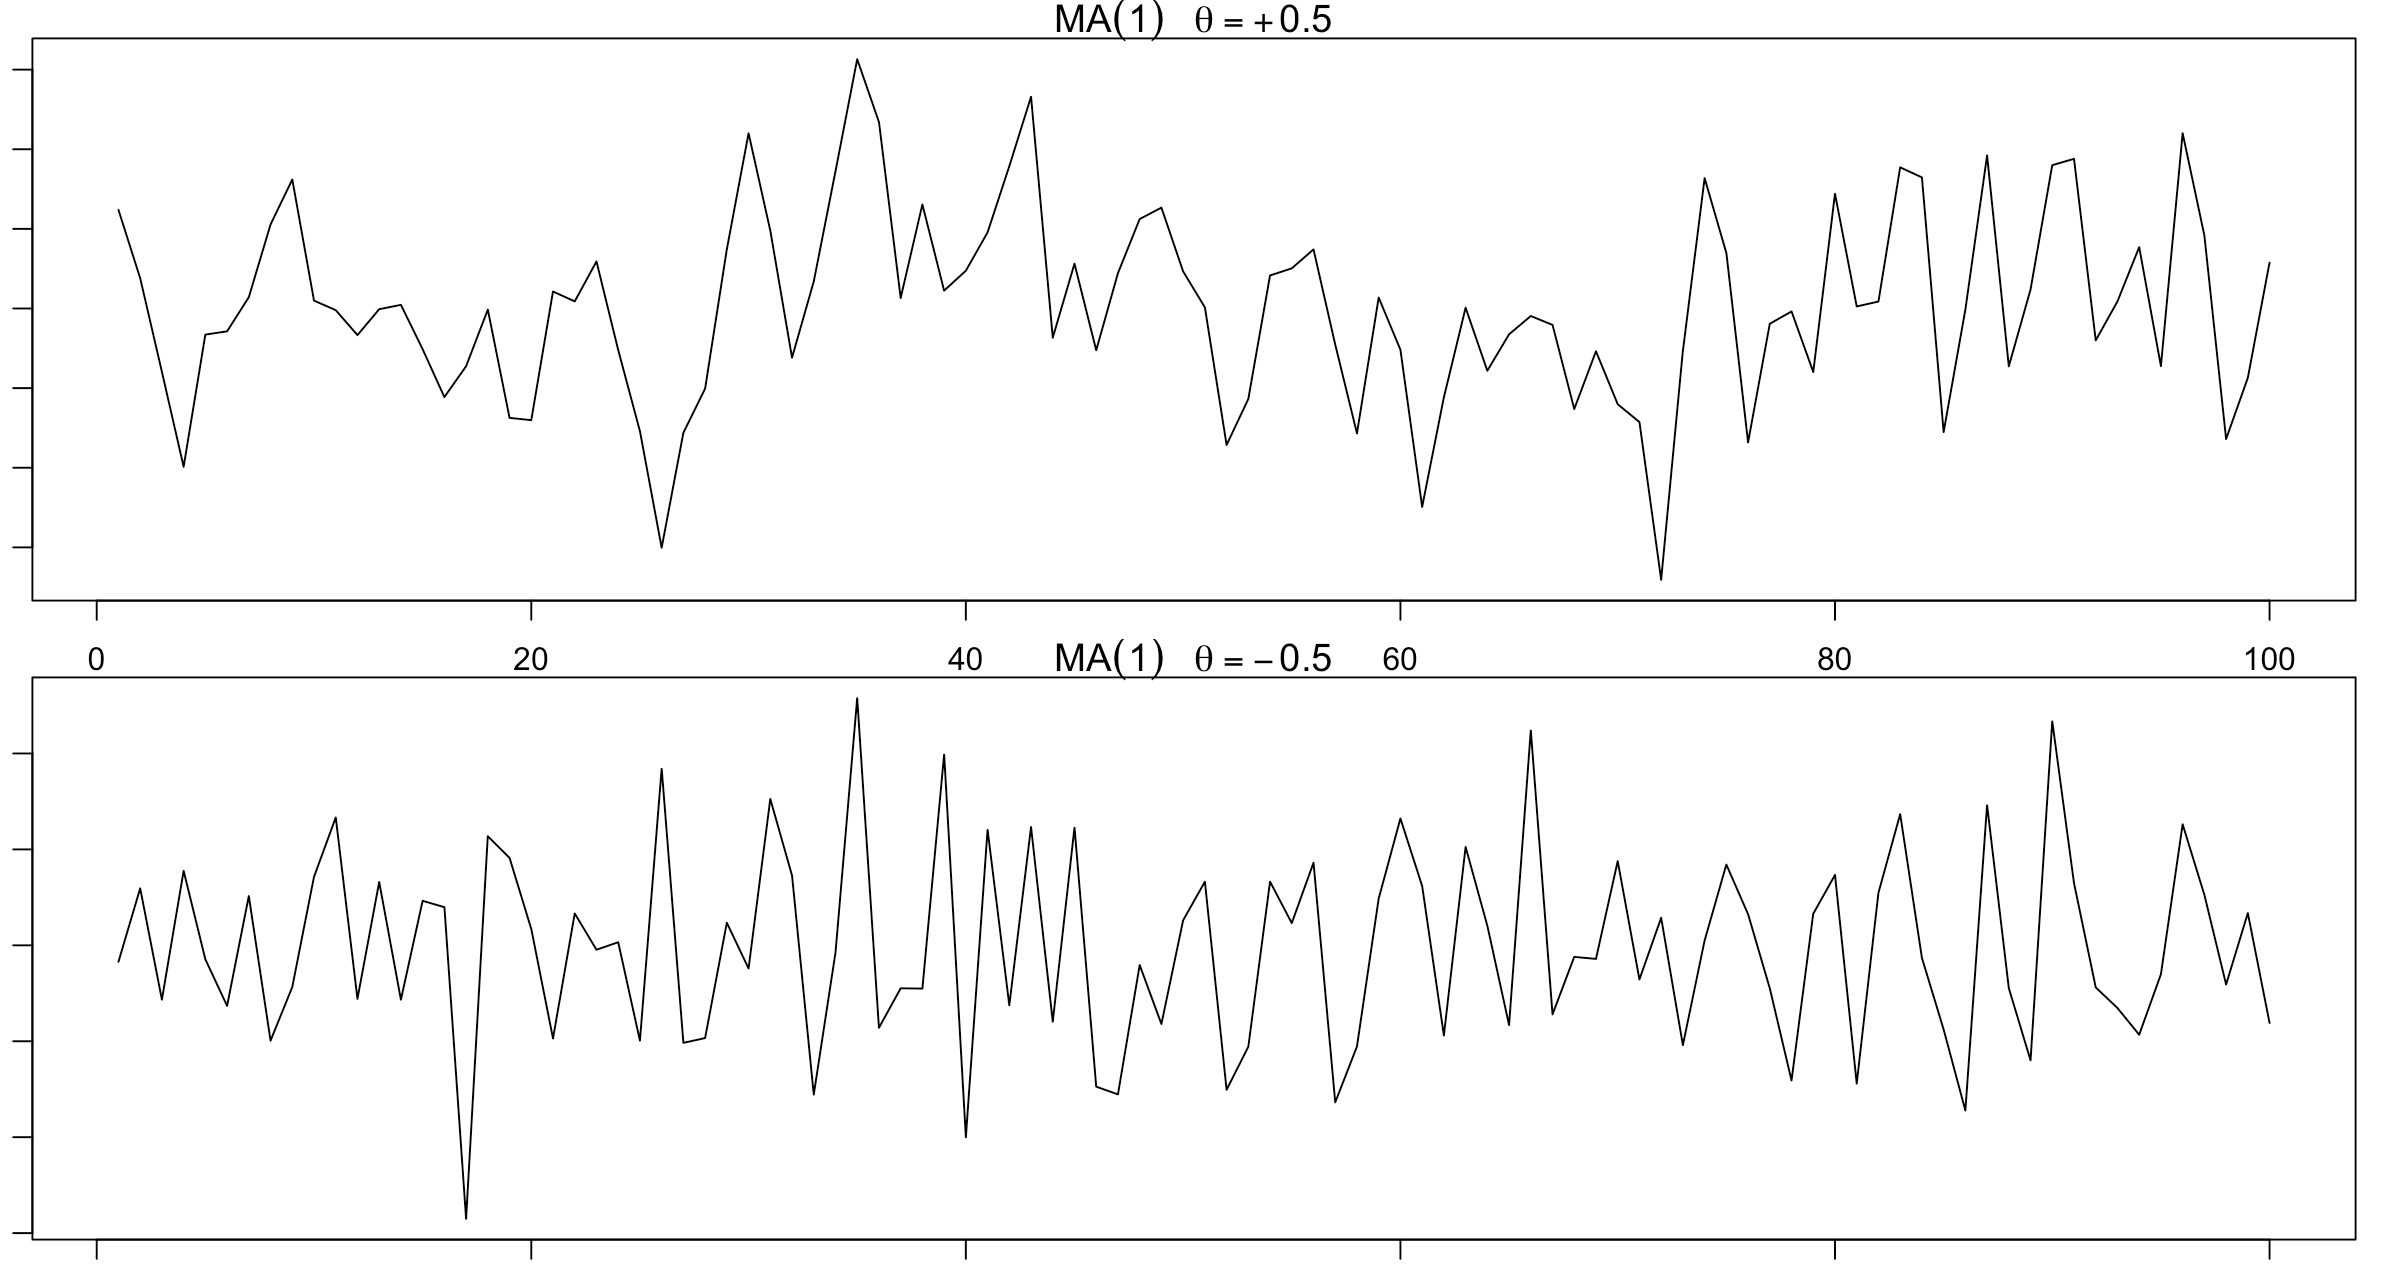
\includegraphics[scale=0.25]{ma.png}
\end{figure}
 
\end{frame}

%---------------------------------------------------------
%---------------------Slide 38--------------------------
\begin{frame}
\frametitle{Identificaci\'on modelo MA }

Para la identificaci\'on de todos los componentes del modelo MA, tal como vimos para el modelo AR, se utiliza la funci\'on de autocorrelaci\'on (AFC) y la funci\'on de autocorrelaci\'on parcial (PAFC), y as\'{\i} se procede a la identificaci\'on de los componentes, en base a los gr\'aficos de los distintos modelos te\'oricos.

\begin{figure}[t!]
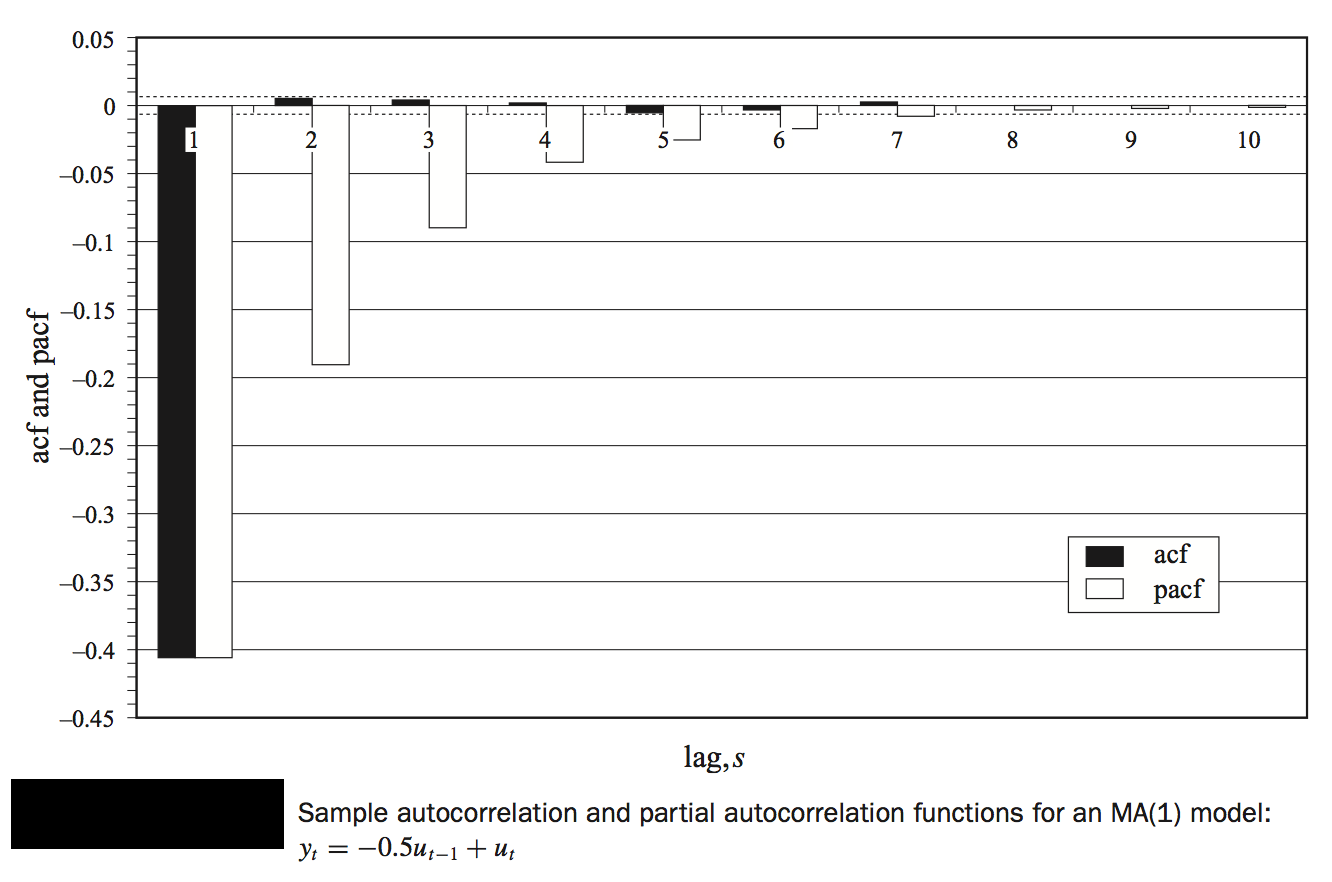
\includegraphics[scale=0.3]{idMA1.pdf}
\end{figure}


\end{frame}
%---------------------------------------------------------
%---------------------Slide 39--------------------------
\begin{frame}
\frametitle{Identificaci\'on modelo ARMA }


\begin{figure}[t!]
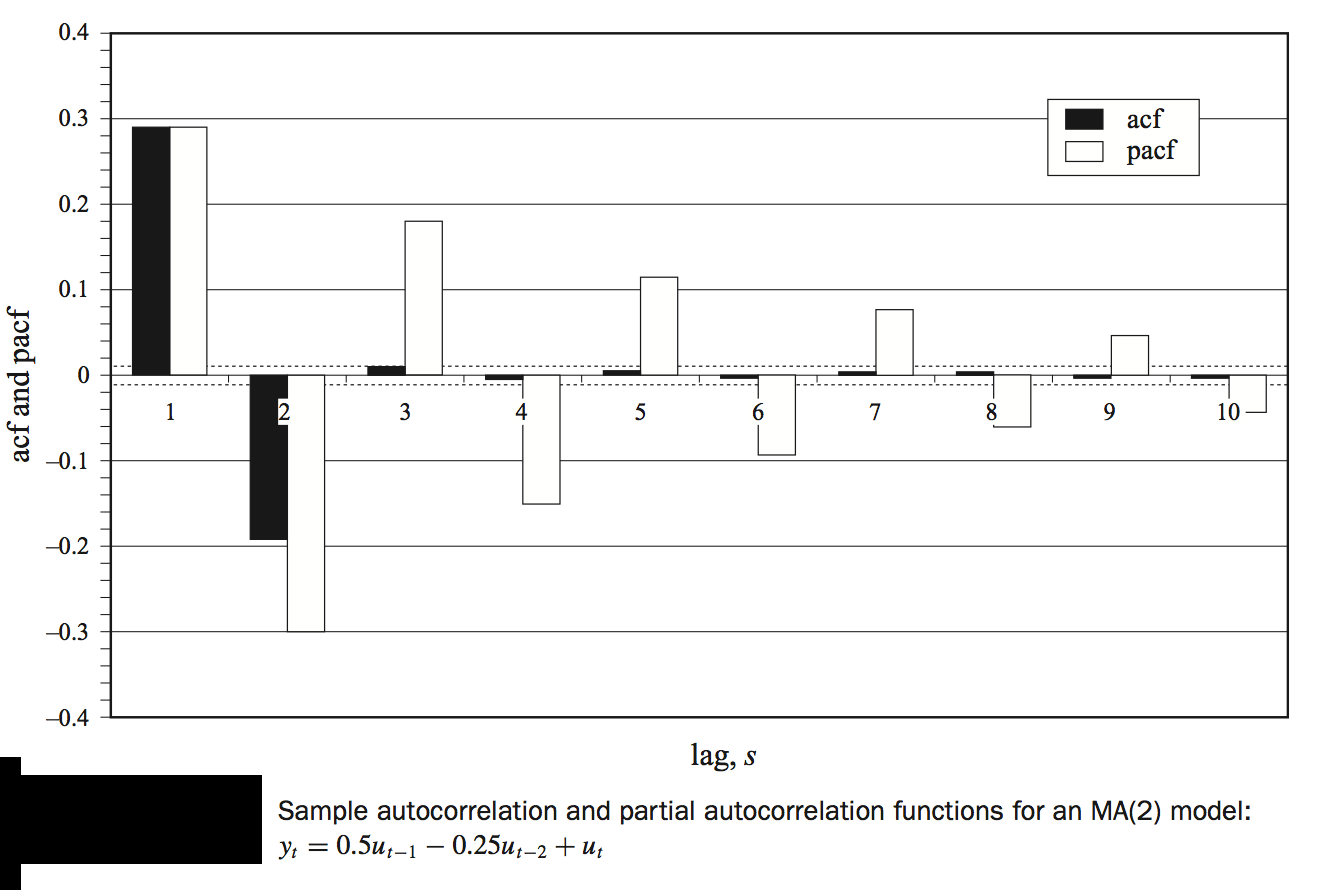
\includegraphics[scale=0.4]{idMA2.pdf}
\end{figure}


\end{frame}
%---------------------------------------------------------
%---------------------Slide 40--------------------------
\begin{frame}
\frametitle{Modelos ARIMA: modelando el corto plazo}

\only<1|handout:1>{
\begin{block}{Definici\'on: Modelo ARMA - $ARMA (r,q)$}

Una serie de tiempo $\{x_t, t = 0, \pm1, \pm2 , \dots{} \}$ es un proceso ARMA(p, q), si es estacionario y	
\begin{equation}
x_t =  \phi_1 x_{t-1} +  \phi_2 x_{t-2} + \dots{} +  \phi_p x_{t-p} + \epsilon_t + \theta_1 \epsilon_{t-1} +  \theta_2 \epsilon_{t-2} + \dots{} +  \theta_q \epsilon_{t-q} 
\end{equation}

Los par\'ametros p y q se llaman \'ordenes autoregresivas y promedios m\'oviles, respectivamente. \\
\vspace{4mm}	
Si $x_t$ tiene una media distinta de cero $\mu$, establecemos que $\alpha = \mu (1-\theta_1, \dots{} -\theta_q)$ y podemos re-escribimos el modelo como:

\begin{equation}
x_t = \alpha + \phi_1 x_{t-1} + \dots{} + \phi_p x_{t-p} + w_t +\theta_1  \epsilon_{t-1} + \dots{} + \theta_q  \epsilon_{t-q} .
\end{equation}

\end{block}
}
 
\end{frame}

%---------------------------------------------------------
%---------------------Slide 41 --------------------------
\begin{frame}
\frametitle{Modelos ARIMA: modelando el corto plazo}

\textbf{Invertibilidad}
Una serie temporal es invertible si los errores se pueden invertir en una representaci\'on de observaciones pasadas. As\'{\i} por ejemplo, como ya vimos, el modelo AR es siempre invertible.
En el caso del modelo ARMA, las ra\'{\i}ces de las siguientes ecuaciones deben ser analizadas para garantizar invertibilidad.

\begin{equation}
\phi (z) = 1 + \phi_1 z + \phi_2 z^2 + \dots{} + \phi_p z^p
\end{equation}

\begin{equation}
\theta(z) =  1 + \theta_1 z + \theta_2 z^2 + \dots{} + \theta_q z^q
\end{equation}

En particular el modelo ARMA ser\'a invertible si y solo si $\theta(z) \ne 0$ para $|z| \le 1$
En general, los valores propios son la soluci\'on del $det (A - \lambda I)$ = 0, vemos que este es casi el polinomio caracter\'{\i}stico de las ecuaciones que definimos arriba. Por lo tanto, vemos que los valores propios de A son el inverso de las ra\'{\i}ces del polinomio caracter\'{\i}stico, y esa convergencia de la iteraci\'on hacia atr\'as ocurre cuando las ra\'{\i}ces del polinomio caracter\'{\i}stico se encuentran fuera del c\'{\i}rculo unitario.

\end{frame}
%---------------------------------------------------------
%---------------------Slide 42 --------------------------
\begin{frame}
\frametitle{Modelos ARIMA: modelando el corto plazo}

\textbf{Estacionaridad e Invertibilidad}
Wold demostr\'o que todos los procesos estoc\'asticos estacionarios de covarianza podr\'{\i}an descomponerse como la suma de
procesos determin\'{\i}sticos y linealmente indeterministas los cuales no estaban correlacionados con todos los rezagos; es decir,
si $y_t$ es la covarianza estacionaria, entonces:

\begin{equation}
y_t = x_t + z_t
\end{equation}

donde $x_t$ es un proceso determinista estacionario en covarianza y $z_t$ es linealmente indeterminista,
con $Cov (x_t, z_s) = 0$ para todas los $t$ y $s$. Este resultado proporciona una base te\'orica para la propuesta de Box y Jenkins  para modelar procesos estacionarios de covarianza escalar (desestacionalizados) como son los procesos ARMA.
\end{frame}
%---------------------------------------------------------
%---------------------Slide 43--------------------------
\begin{frame}
\frametitle{Modelos ARIMA: modelando el corto plazo}

\textbf{Modelos ARMA (p,q)}

Como se indic\'o anteriormente, cuando $q$ = 0, el modelo se denomina modelo autoregresivo de orden $p$, $AR (p)$, y cuando $p$ = 0, el modelo se denomina modelo de promedio m\'ovil de orden $q$, $MA (q)$. \\
Es \'util escribir los modelos ARIMA usando el operador AR y el operador MA descritos anteriormente. En particular, el modelo $ARMA (p, q) $ puede escribirse entonces en forma concisa como:

\begin{equation}
\phi (B) x_t = \theta (B) \epsilon_t.
\end{equation}
\textbf{Modelos ARIMA (p, i, q)}
El modelo ARMA gana su I y se convierte en ARIMA cuando debe ser integrado para lograr estacionaridad. El \'{\i}ndice $I$ ser\'a entonces el numero de veces que debe ser diferenciado.
\end{frame}

%---------------------------------------------------------
%---------------------Slide 44--------------------------
\begin{frame}
\frametitle{Identificaci\'on modelo ARMA }

Para la identificaci\'on de todos los componentes del modelo ARMA se utiliza la funci\'on de autocorrelaci\'on (AFC) y la funci\'on de autocorrelaci\'on parcial (PAFC), y as\'{\i} se procede a la identificaci\'on de los componentes estacional y no estacional por separado, en base a los gr\'aficos de los distintos modelos te\'oricos.

\begin{figure}[t!]
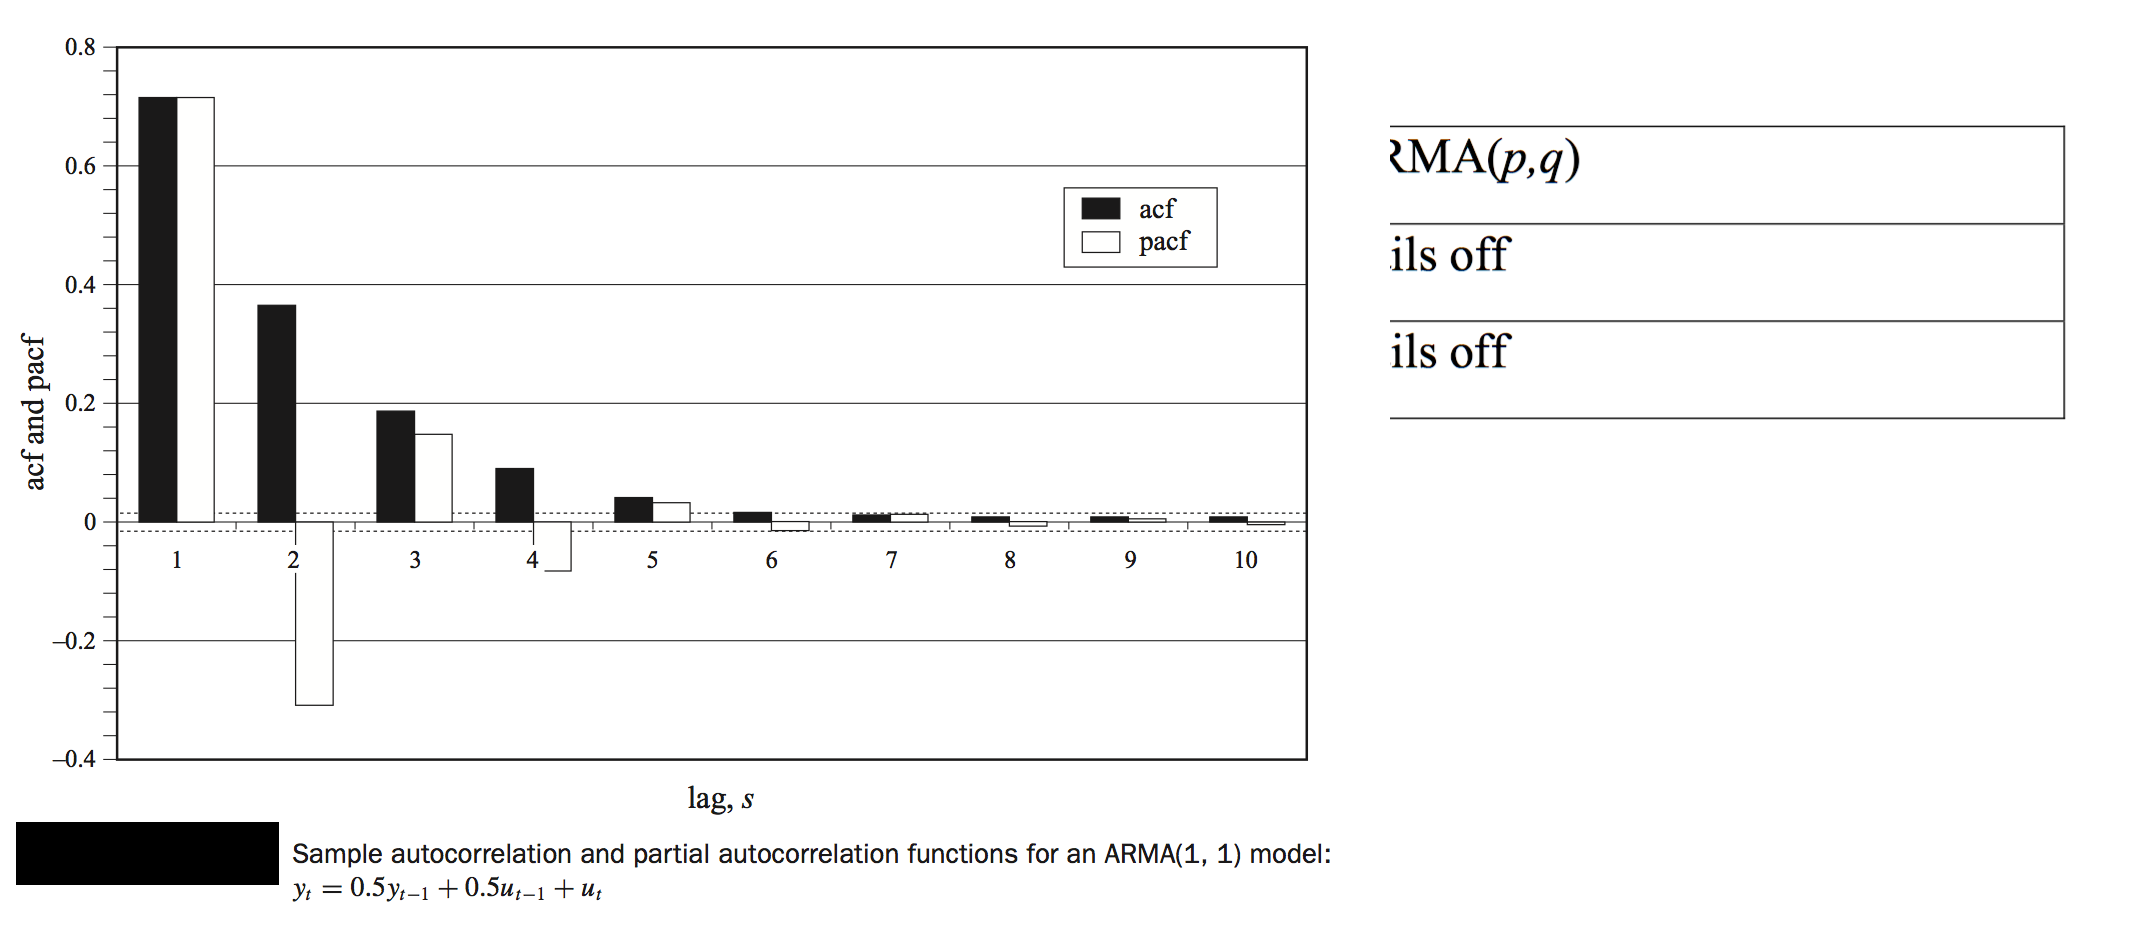
\includegraphics[scale=0.3]{idARMA.pdf}
\end{figure}

\end{frame}
%---------------------------------------------------------
%---------------------Slide 45--------------------------
\begin{frame}
\frametitle{Identificaci\'on modelo ARMA }

En resumen tendremos:

\begin{figure}[t!]
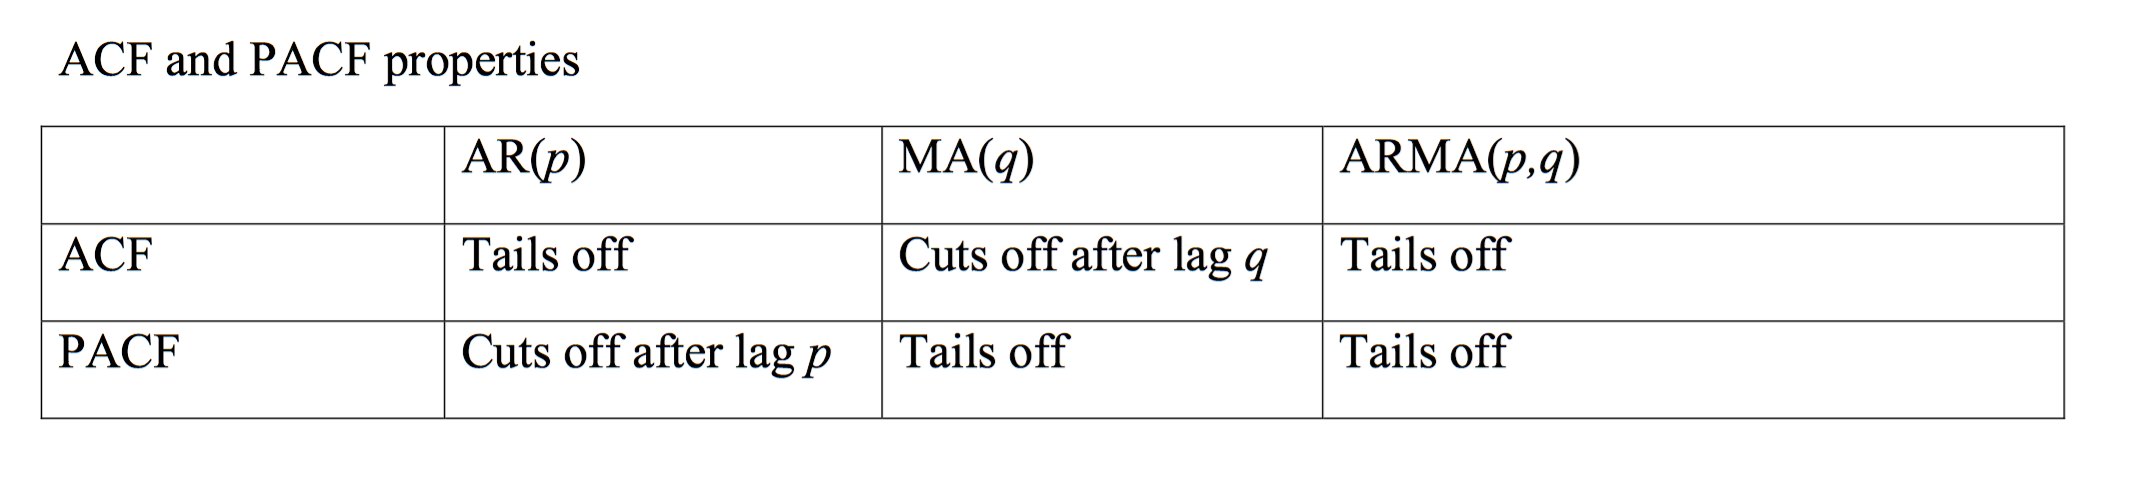
\includegraphics[scale=0.5]{resumenARMA.pdf}
\end{figure}

\end{frame}
%---------------------------------------------------------
%---------------------Slide 46--------------------------
\begin{frame}
\frametitle{Modelos SARIMA (p,q)}

Los modelos ARIMA tambi\'en son capaces de modelar una amplia gama de datos estacionales. Los llamados  modelos SARIMA, Seasonal ARIMA models, se obtienen al incluir t\'erminos estacionales adicionales en los modelos ARIMA que hemos visto hasta ahora, de la siguiente manera:

\begin{equation}
ARIMA (p,d,q)(P,D,Q)m
\end{equation}

donde m = n\'umero de per\'{\i}odos por temporada. \\
Usamos la notaci\'on en may\'usculas para las partes estacionales del modelo y la notaci\'on en min\'usculas para las partes no estacionales del modelo.\\
La parte estacional del modelo consiste en t\'erminos que son muy similares a los componentes no estacionales del modelo, pero implican retrocesos del per\'{\i}odo estacional. \\

\end{frame}
\end{section}
%---------------------------------------------------------
%---------------------Slide 47--------------------------
\begin{section}{Evaluaci\'on estad\'{\i}stica de un Modelo ARIMA}
\begin{frame}
\frametitle{Evaluaci\'on estad\'{\i}stica de un Modelo ARIMA}
Se debe evaluar:
\only<1->{
\begin{itemize}
\item[A] \textbf{Significancia estad\'{\i}stica de los par\'ametros} 
Los coeficientes obtenidos en la estimaci\'on que no sean significativamente distintos de cero, a un nivel de significancia del $5\%$, no son necesarios, por lo que deben eliminarse.
\item[B] \textbf{Estacionariedad e invertibilidad del modelo estimado.} Para valores de los coeficientes estimados pr\'oximos a la frontera de la no-estacionariedad, es conveniente llevar a cabo un test de ra\'{\i}ces unitarias.
\item[C] \textbf{Estabilidad del modelo estimado.} Aunque los par\'ametros sean significativos, el modelo puede ser rechazado si existe una fuerte correlaci\'on entre los par\'ametros del modelo. Esto ocurre cuando el coeficiente de correlaci\'on tiene un valor absoluto superior a 0,7, entonces es conveniente probar con modelos alternativos.
\end{itemize}
} 
 
\end{frame}

%---------------------------------------------------------
%---------------------Slide 48--------------------------
\begin{frame}
\frametitle{Sobre la Selecci\'on de Modelos}

Puede ocurrir que varios modelos describan satisfactoriamente la serie temporal, por lo que sea necesario seleccionar el modelo m\'as adecuado. Este proceso de selecci\'on puede ser sencillo o un poco m\'as complejo, por lo que es necesario recurrir a criterios de selecci\'on de modelos.
\par
Los criterios m\'as comunes en la selecci\'on de modelos son el AIC (Akaike Information Criterion) y el BIC (Bayesian Information Criterion) que es una extensi\'on bayesiana del primero. 

\end{frame}

%---------------------------------------------------------
%---------------------Slide 49 --------------------------
\begin{frame}
\frametitle{Criterios de Informaci\'on}

\only<1|handout:1>{
\begin{block}{Definici\'on: Akaike Information Criterion}
\begin{equation*}
AIC = log \hat{\sigma_k^2} + \frac{n+2k}{n} 
\end{equation*}
\end{block}
}
\vspace{4mm}	
Donde $\hat{\sigma_k^2} = \frac{SSE_k}{n}$, donde $k$ es el n\'umero de par\'ametros del modelo, $n$ el tama\~no de la muestra, y $SSE_k$ equivale a la suma de los residuos al cuadrado bajo el modelo $k$ ($SSE_k=\sum_{t=1}^{n}(x_t-\bar{x})^2$). 
\par
\vspace{4mm}	
El valor de $k$ que produce el m\'{\i}nimo AIC representa el mejor modelo. La idea es que minimizar $\hat{\sigma_k^2}$ representa un objetivo razonable, excepto que disminuye mon\'otonamente a medida que $k$ aumenta. Por lo tanto, debemos penalizar la varianza del error por un t\'ermino proporcional al n\'umero de par\'ametros.

\end{frame}

%---------------------------------------------------------
%---------------------Slide 50 --------------------------
\begin{frame}
\frametitle{Criterios de Informaci\'on}

\only<1|handout:1>{
\begin{block}{Definici\'on: Bias Corrected}
\begin{equation*}
AICc = log \hat{\sigma_k^2} + \frac{n+k}{n-k-2} 
\end{equation*}
\end{block}
}

\only<1|handout:1>{
\begin{block}{Definici\'on: Bayesian Information Criterion - BIC}
\begin{equation*}
AICc = log \hat{\sigma_k^2} + \frac{k log n}{n} 
\end{equation*}
\end{block}
}
BIC tambi\'en se conoce como el \textbf{Schwarz Information Criterion (SIC)}. Varios estudios de simulaci\'on han verificado que BIC es adecuado para obtener el orden correcto en muestras grandes, mientras que AICc tiende a ser superior en muestras m\'as peque\~nas donde el n\'umero relativo de par\'ametros es grande.

\end{frame}

%---------------------------------------------------------
%---------------------Slide 51--------------------------
\begin{frame}
\frametitle{Sobre la Selecci\'on de Modelos}

En \'ultimo t\'ermino un modelo es mejor que otro si su predicci\'on es mejor. Por otro lado, diremos que \textbf{una predicci\'on, es mejor que otra, cuando comete un menor error extra-muestral.} 
\par
As\'{\i}, la precisi\'on de los m\'etodos utilizados para pronosticar se pueden medir por ejemplo a trav\'es de la funci\'on de p\'erdida: \textbf{Error cuadr\'atico medio - Mean Square Error (MSE)}, con el fin de comprender qu\'e modelo proporciona un mejor pron\'ostico extra-muestral sobre otro. Esto es:

\begin{equation}
\textbf{MSE}=\frac{1}{T} \sum_{t=1}^T (x_t-\hat{x}_t)^2
\label{MSE}
\end{equation}

donde $x_t$ corresponde al valor real de la serie en el tiempo $t$ y $\hat{x}_{t}$ corresponde al valor pronosticado por el modelo propuesto en el mismo instante.
 
\end{frame}

%---------------------------------------------------------
%---------------------Slide 52--------------------------
\begin{frame}
\frametitle{Sobre la Selecci\'on de Modelos}

Otros criterios de selecci\'on de modelos que consideran el error extra-muestral son: i) el \textbf{Error Absoluto Medio (EAM) - mean absolute deviation (MAD)}, y ii) \textbf{Error Absoluto Porcentual Medio (EAPM) - mean absolute percentage error (MAPE)}. 
 
 \begin{equation}
\textbf{MAD}=\frac{1}{T} \sum_{t=1}^T |x_t-\hat{x}_t|
\label{MAD}
\end{equation}

 \begin{equation}
\textbf{MAPE}=\frac{1}{T} \sum_{t=1}^T \left| 1 - \frac{x_t}{\hat{x}_t}\right|
\label{MAPE}
\end{equation}
\end{frame}

%---------------------------------------------------------
%---------------------Slide 53 --------------------------
\begin{frame}
\frametitle{Ejemplo IPC en Chile}

Considerando data mensual del IPC desde enero del 2013 a la fecha en Chile, obtenida de la p\'agina del Banco Central, intetnaremos predecir el IPC (serie original).
\only<1|handout:1>{
\begin{exampleblock}{C\'odigo en R}
rm(list=ls())\\
data$<-$read.csv (``ipc.csv")\\
ipc $<-$ ts(data[,2],start = c(2013,1), end=c(2018, 6), frequency = 12)\\
plot.ts(ipc, xlab='Years', ylab = ``Indice de Precios al Comsumidor')\\

\end{exampleblock}
}

\end{frame}
%---------------------------------------------------------
%---------------------Slide 54--------------------------
\begin{frame}
\frametitle{Ejemplo IPC en Chile}

\begin{figure}[t!]
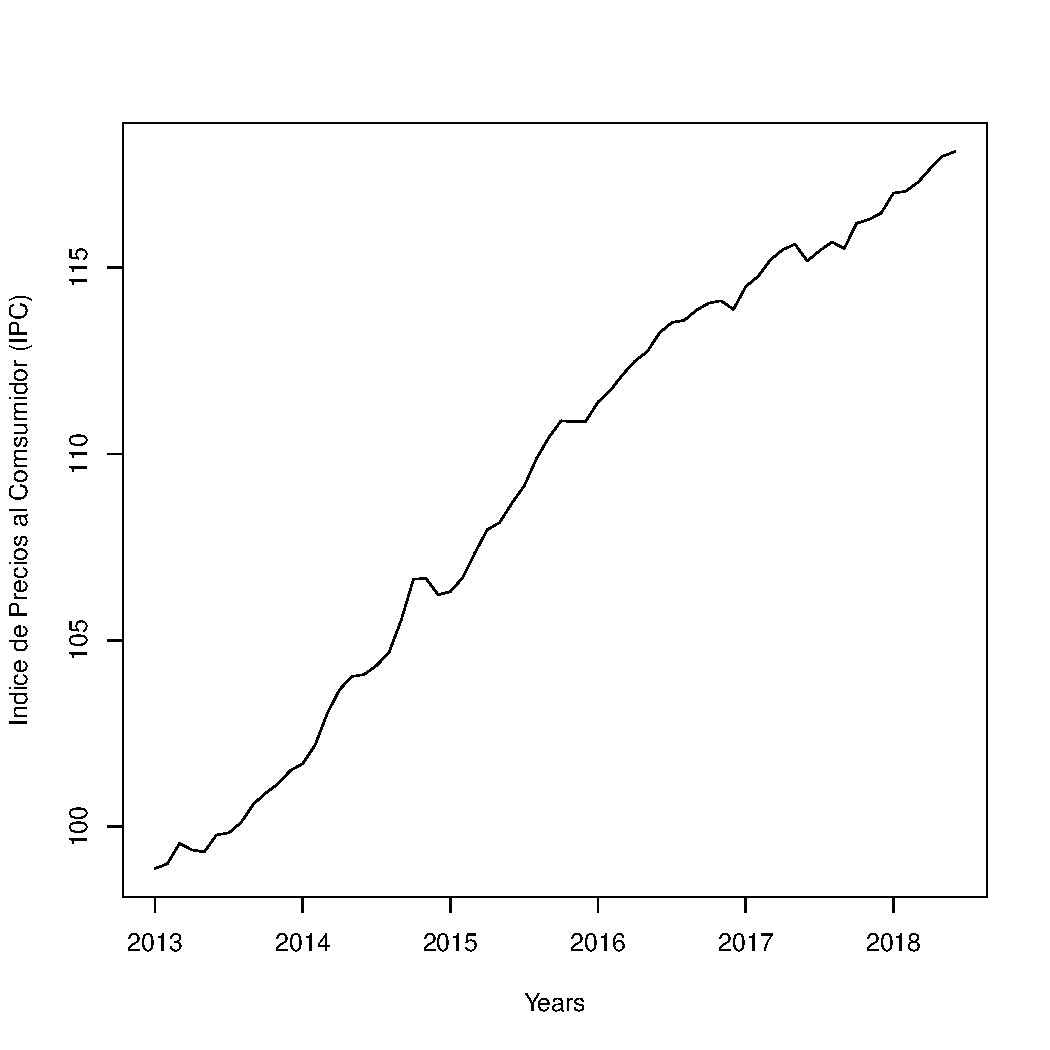
\includegraphics[scale=0.3]{ipc.pdf}
\end{figure}
 
\end{frame}

%---------------------------------------------------------
%---------------------Slide 55 --------------------------
\begin{frame}
\frametitle{Ejemplo IPC en Chile}
Encontrando el orden del modelo. Tendencia, estacionaridad, autocorrelaci\'0n.
\only<1|handout:1>{
\begin{exampleblock}{C\'odigo en R}

$\#$ Descomposici\'on\\
fit $<-$ stl(ipc, s.window=``period")\\
plot(fit)\\

$\#$ Test de ra\'{\i}z unitaria\\
adf.test(ipc)\\
adf.test(diff(ipc))\\

$\#$ Funci\'on de autocorrelaci\'on (AFC) y autocorrelaci\'on parcial (PAFC)\\
acf(diff(ipc),lag=36,lwd=3)\\
pacf(diff(ipc),lag=36,lwd=3)\\
\end{exampleblock}
}

\end{frame}
%---------------------------------------------------------
%---------------------Slide 56--------------------------
\begin{frame}
\frametitle{Ejemplo IPC en Chile}

\textbf{Descomposici\'on\ de la serie}\\

\begin{figure}[t!]
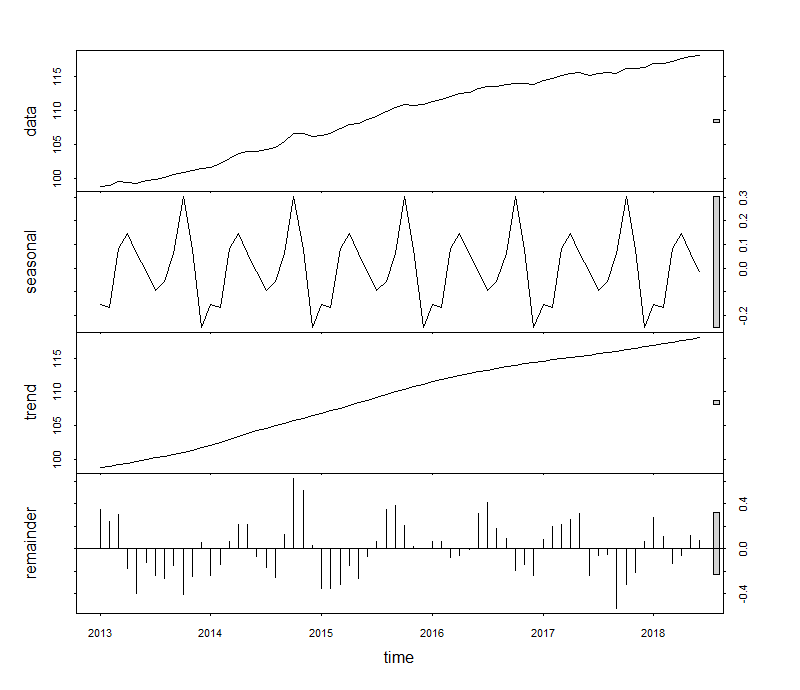
\includegraphics[scale=0.125]{ipcdecomp.png}
\end{figure}
 
\end{frame}

%---------------------------------------------------------
%---------------------Slide 57--------------------------
\begin{frame}
\frametitle{Ejemplo IPC en Chile}

\textbf{Test de ra\'{\i}z unitaria}\\
\vspace{4mm}	
Augmented Dickey-Fuller Test\\
data:  ipc\\
Dickey-Fuller = -0.11148, Lag order = 4, p-value =0.99\\
alternative hypothesis: stationary\\
 \vspace{4mm}	
 Augmented Dickey-Fuller Test\\
data:  diff(ipc)\\
Dickey-Fuller = -5.8024, Lag order = 3, p-value = 0.01\\
alternative hypothesis: stationary\\

\end{frame}

%---------------------------------------------------------
%---------------------Slide 58--------------------------
\begin{frame}
\frametitle{Ejemplo IPC en Chile}

\textbf{Funci\'on de autocorrelaci\'on (AFC) y autocorrelaci\'on parcial (PAFC)}\\
\begin{figure}[t!]
\includegraphics[scale=0.25]{acfipc.pdf}
\includegraphics[scale=0.25]{pacfipc.pdf}
\end{figure}
 
\end{frame}

%---------------------------------------------------------
%---------------------Slide 59--------------------------
\begin{frame}
\frametitle{Ejemplo IPC en Chile}

\textbf{Pron\'ostico.}\\
 \vspace{4mm}	
\only<1|handout:1>{
\begin{exampleblock}{C\'odigo en R}

train.series =ipc $\left [ 1:44 \right ]$\\
test.series = ipc $\left [ 45:62 \right ]$\\
arima.model=arima(train.series, order=c(0,1,1))\\
forecast=predict(arima.model, length(test.series)\\

mse $<-$sum((forecast$\$$pred-test.series)$\wedge2$)/length(test.series)\\
mad $<-$ sum(abs(forecast$\$$pred-test.series))/length(test.series)\\
mape $<-$ sum(abs( 1 - forecast$\$$pred/test.series))/length(test.series)\\

fit $<-$ auto.arima(ipc)\\
summary(fit)\\
plot(fit)\\
mape $<-$ sum(abs(1 - test.series/f$[[``mean"]])$)/length(test.series)\\
accuracy(fit)\\
\end{exampleblock}
}

\end{frame}
%---------------------------------------------------------
%---------------------Slide 60--------------------------
\begin{frame}
\frametitle{Ejemplo IPC en Chile}
\textbf{output ARIMA (0, 1, 1) }\\
 \vspace{4mm}	
Call:\\
arima(x = train.series, order = c(0, 1, 1))\\

Coefficients:\\
\hspace{3em}ma1\\
\hspace{2.5em}$0.8205$\\
s.e.\hspace{1em}$ 0.0906$\\

$\sigma^2$ estimated as $0.1029:  log likelihood = -12.68,  aic = 29.37$\\
 \vspace{4mm}
\textbf{forecast ARIMA (0, 1, 1) }\\
mse
[1] 69.80031
\end{frame}

%---------------------------------------------------------
%---------------------Slide 61--------------------------
\begin{frame}
\frametitle{Ejemplo IPC en Chile}
\textbf{Pron\'ostico - output ARIMA (0, 1, 1) }\\
 \vspace{4mm}	
$\$$pred\\
Time Series:\\
Start = 45 \\
End = 54 \\
Frequency = 1 \\
$\left [ 1 \right ]$ $113.6141$ $113.6253$ $113.6292$ $113.6307$ $113.6311$ $113.6313$\\
$\left [ 7 \right ]$ $113.6314$ $113.6314$ $113.6314$ $113.6314$\\

$\$$se\\
Time Series:\\
Start = 45 \\
End = 54 \\
Frequency = 1 \\
$\left [ 1 \right ]$ $0.3128668$ $0.6841962$ $0.9882296$ $1.2406559$ $1.4565974$\\
$\left [ 6 \right ]$ $1.6465783$ $1.8174943$ $1.9738906$ $2.1188485$ $2.2545301$\\

\end{frame}

%---------------------------------------------------------
%---------------------Slide 62--------------------------
\begin{frame}
\frametitle{Ejemplo IPC en Chile}
\textbf{output auto.arima}\\

Series: ipc \\
ARIMA(0,1,1)(0,0,1)[12] with drift \\
 \vspace{2mm}	
Coefficients:\\
\hspace{5em}ma1\hspace{3em}sma1\hspace{3em}drift\\
\hspace{5em}$0.2329$\hspace{2em}$0.2483$\hspace{2em}$0.2909$\\
s.e.\hspace{3.5em}$0.1443$\hspace{2em}$0.1396$\hspace{2em}$0.0500$\\
 \vspace{2mm}	
$\sigma^2$ estimated as $0.07771:  log likelihood=-8.01$\\
$AIC=24.02$  $ ICc=24.69$  $BIC=32.72$\\
 \vspace{2mm}	
Training set error measures:\\
\hspace{7em}ME\hspace{2em}RMSE\hspace{3em}MAE\hspace{2em}MPE\\
Training set $0.00467571$ $0.2701877$ $0.2012356$ $0.005434612$\\
\hspace{7em}MAPE\hspace{2em}MASE\hspace{2em}ACF1\\
Training set $0.185618$ $0.05414794$ $-0.03368001$\\

\end{frame}

%---------------------------------------------------------
%---------------------Slide 63--------------------------
\begin{frame}
\frametitle{Ejemplo IPC en Chile}
\textbf{Inverse MA roots  - auto.arima}\\
 \vspace{4mm}	
\begin{figure}[t!]
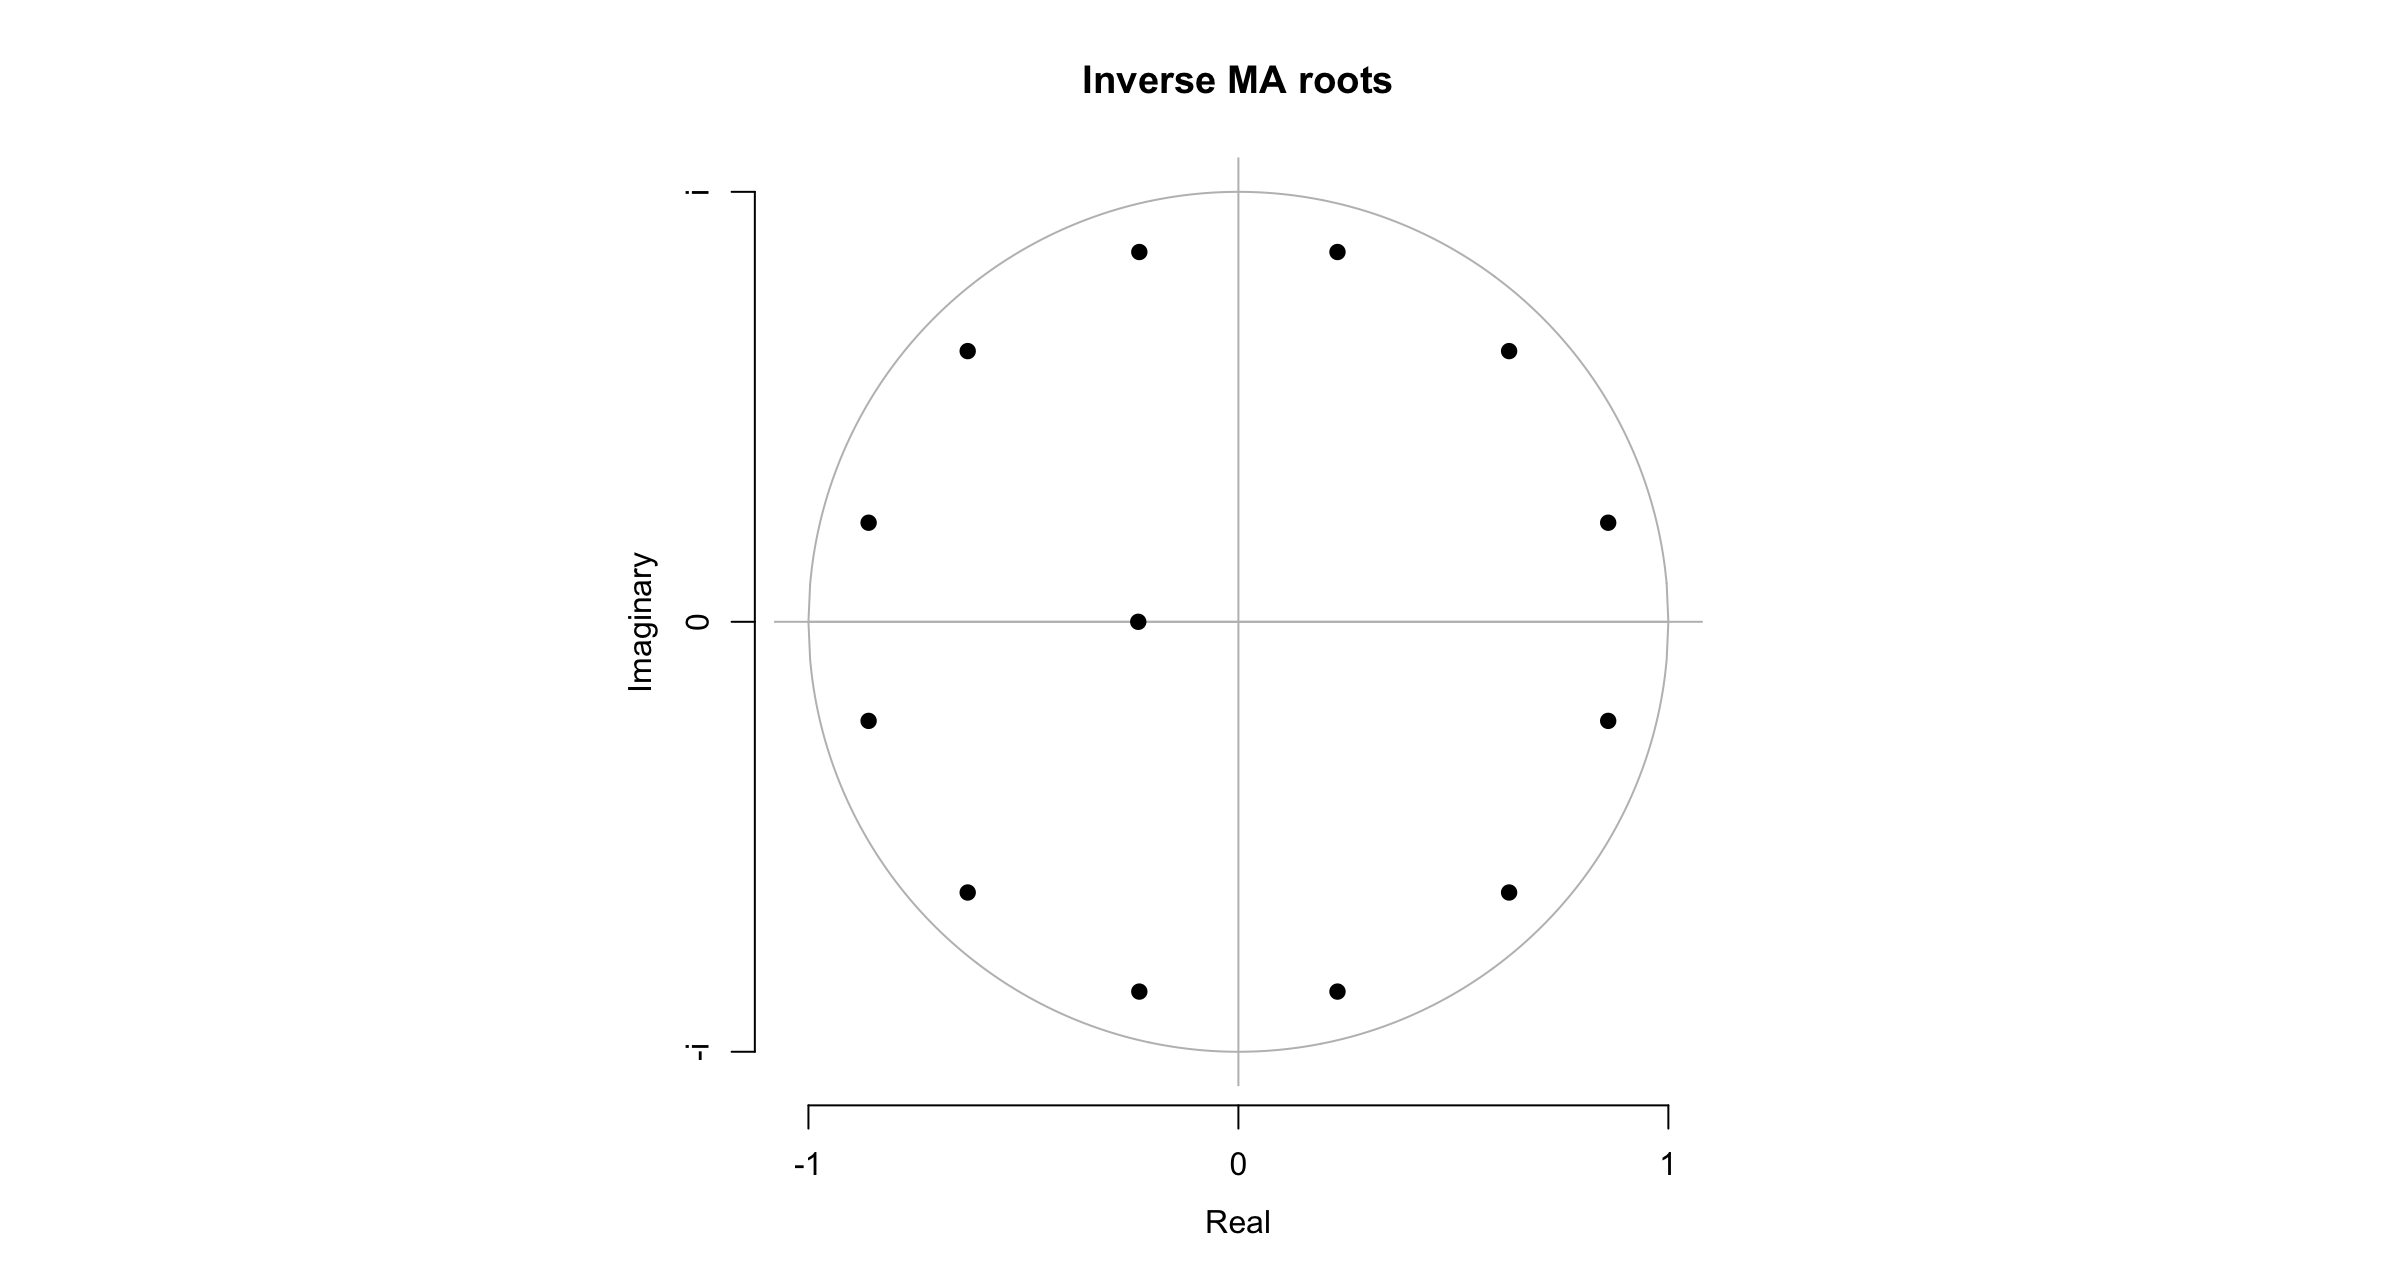
\includegraphics[scale=0.12]{maroots.png}
\end{figure}
 
\end{frame}

%---------------------------------------------------------
%---------------------Slide 64--------------------------
\begin{frame}
\frametitle{Ejemplo IPC en Chile}
\textbf{Pron\'ostico auto.arima}\\
 \vspace{4mm}	
\begin{figure}[t!]
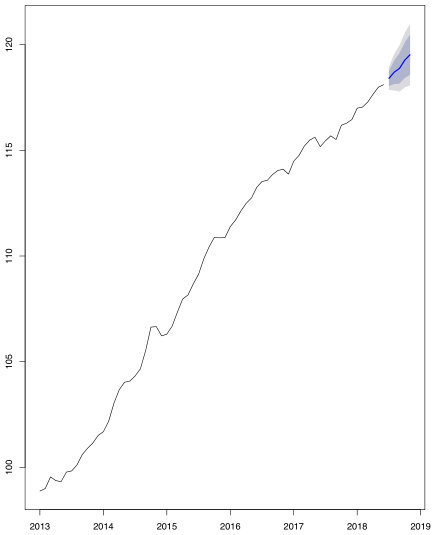
\includegraphics[scale=0.25]{forecastipc.pdf}
\end{figure}
 
\end{frame}
\end{section}
%---------------------------------------------------------
%---------------------Slide 65--------------------------
\begin{section}{Metodolog\'{\i}a de Estimaci\'on de un Modelo ARIMA}
\begin{frame}
\frametitle{Etapas de Estimaci\'on de un Modelo ARIMA}

\only<1->{
\begin{itemize}
\item[1] \textbf{Recolecci\'on de datos}: Es recomendable disponer de a lo menos 50 datos, y en el caso de series mensuales, es conveniente trabajar con entre seis y diez a\~nos de datos.
\item[2] \textbf{Representaci\'on gr\'afica de la serie}: Resulta de gran utilidad disponer de diversos gr\'aficos de la serie y sus transfromaciones para decidir sobre la estacionariedad de la misma.
\item[3] \textbf{Transformaci\'on de la serie}: La transformaci\'on de la serie es muchas veces necesaria en caso de encontrarnos con no-estacionaridad.
\item[4] \textbf{Eliminaci\'on de la tendencia}: Al comprobarse gr\'aficamente la existencia de una tendencia, esta debe ser eliminada usando como vimos primeras diferencias, e incluso dos diferencias para una tendencia no lineal.
\end{itemize}
}

 
\end{frame}


%---------------------------------------------------------
%---------------------Slide 66--------------------------
\begin{frame}
\frametitle{Etapas de Estimaci\'on de un Modelo ARIMA}

\only<1->{
\begin{itemize}
\item[5] \textbf{Identificaci\'on del modelo}: Se debe determinar el tipo de modelo m\'as adecuado, es decir, el orden de los procesos autorregresivos y de medias m\'oviles de las componentes regular y estacional. Se suelen seleccionar varios modelos alternativos, estimarlos, y contrastarlos, antes de modelar definitivamente la serie.
\item[6] \textbf{Estimaci\'on de los coeficientes del modelo}: A partir del modelo elegido se procede a la estimaci\'on de sus par\'ametros.
\item[7] \textbf{Contraste de validez conjunta del modelo}: Se utilizan los diversos criterios y procedimientos vistos anteriormente para valorar el modelo o modelos seleccionados: test de significancia de par\'ametros, criterios de informaci\'on, covarianzas entre estimadores, coeficiente de correlaci\'on, $R^2$, i.e. suma de cuadrados de errores, etc.
\end{itemize}
}
 
\end{frame}

%---------------------------------------------------------
%---------------------Slide 67--------------------------
\begin{frame}
\frametitle{Etapas de Estimaci\'on de un Modelo ARIMA}

\only<1->{
\begin{itemize}
\item[8] \textbf{An\'alisis detallado de los errores}: Los errores extra-muestrales del modelo son determinantes para una valoraci\'on final del modelo. Las diferencias entre valores reales y estimados por el modelo son determinantes para una evaluaci\'on final del modelo.
\item[9] \textbf{Selecci\'on del modelo}: Analizando los resultados de las fases anteriores se decidir\'a sobre el modelo adoptado. Si ninguno de los modelos estudiados nos proporciona resultados suficientemente satisfactorios se vuelve a la etapa 3, revisando todas las decisiones adoptadas.
\item[10] \textbf{Predicci\'on}: Se tomar\'a el modelo v\'alido como f\'ormula inicial de predicci\'on. Ser\'a necesario comparar las predicciones con los valores ya conocidos y, posteriormente, analizar los errores extramuestrales.
\end{itemize}
}
 
\end{frame}

%---------------------------------------------------------
%---------------------Slide 68--------------------------
\begin{frame}
\frametitle{Resumen de los pasos de Box-Jenkins}

\begin{figure}[t!]
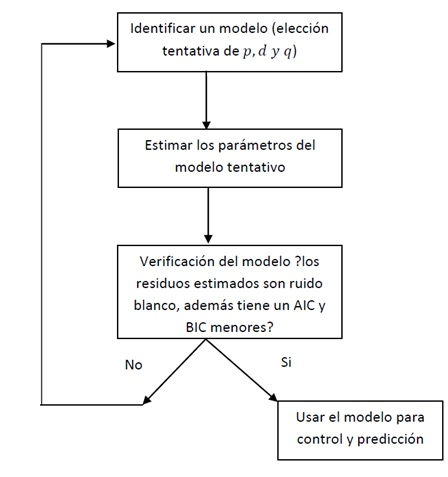
\includegraphics[scale=0.50]{box_jenkins.jpg}
\end{figure}
 
\end{frame}

\end{section}

%---------------------------------------------------------
%---------------------Slide 69--------------------------

\begin{section}{Tarea 2}
\begin{frame}
\frametitle{Tarea 2}
Calibrar y evaluar los siguientes modelos para el precio de un commodity (0 activo en \'ultimo caso) a su eleci\'on:\\
\textbf{1.} Camino aleatorio sin drift., \textbf{2.} Camino aleatorio con drift.\\
\textbf{3.} Promedio de los \'ultimos 5 a\~nos. \textbf{4.} Promedio de los \'ultimos 10 a\~nos. \textbf{5.} ARIMA(1,1,0).\\
\textbf{6.} ARIMA(0,1,1)., \textbf{7.} ARIMA(1,1,1)., \textbf{8.} AR(1)., \textbf{9.} AR(2).,\textbf{10.} AR(3).\\
\textbf{11.} $\alpha$ constante, $\psi$ = 1 y $\delta$ sigue un camino aleatorio.\\
\textbf{12.} $\psi$=1,$\delta$=0 y ?sigue un camino aleatorio.\\
\textbf{13.} $\alpha$ constante, $\delta$ y $\psi$ siguen caminos aleatorios con innovaciones independientes.\\
\textbf{14.} $\delta$ = 0, $\alpha$ y $\psi$ siguen caminos aleatorios con innovaciones independientes. 
\textbf{15.} $\alpha$ constante, $\delta$ = 0 y $\psi$ sigue un camino aleatorio.\\
\textbf{16.} $\alpha$, $\delta$ y $\psi$ siguen caminos aleatorios con innovaciones independientes.\\
\textbf{17.} $\alpha$ constante, $\delta$ = 0 y $\psi$ sigue un AR(1).\\
\textbf{18.} $\alpha$ y $\delta$ constantes, $\psi$ sigue un AR(1).\\
 \vspace{4mm}	
 Basarse en paper anexo.
\end{frame}
\end{section}
%---------------------------------------------------------
%--------------Slide Referencias---------------------

\section{Referencias}
\begin{frame}[allowframebreaks]
        \frametitle{Referencias}
        \bibliographystyle{unsrt}
        \nocite{} %lista sin citar.
        \bibliography{TS_ref}
\end{frame}


%---------------------------------------------------------
%---------------------------------------------------------
\end{document} 
%---------------------------------------------------------




